\documentclass[a4paper, 12pt] {report}

\usepackage[includehead, left=1in, right=1in, top=0.8in, bottom=0.8in]{geometry}
%\usepackage[framemethod=TikZ]{mdframed}
\usepackage{graphicx}
\usepackage{xcolor,colortbl}
\usepackage{listings} % Allows code-listings
%\usepackage{wrapfig}
\usepackage{courier} % proper monospace font for code
%\usepackage{lscape}
\usepackage{rotating}
\usepackage{epstopdf}
\usepackage{hyperref} %linking contents  table
\usepackage{xstring} %string-manipulation
\usepackage{enumitem} %used for enumerate-manipulation
\usepackage{float} %used to properly place float-objects (figures)
\usepackage[T1]{fontenc}
\usepackage{titlesec, blindtext, color}
%\usepackage[norsk]{babel}
\usepackage[utf8]{inputenc}
\usepackage{tabularx,ragged2e,booktabs,caption}
\usepackage{subcaption}
\usepackage{ulem} %used for strikeout
\usepackage{verbatim} %used for block-commenting
\usepackage[toc,page]{appendix}
\usepackage{url}
\usepackage{amsmath}
\usepackage{algorithm}
\usepackage[noend]{algpseudocode}
\usepackage{blindtext}
\usepackage{afterpage}
\usepackage{setspace}
\usepackage{csquotes}
\usepackage[nottoc]{tocbibind}

\usepackage{titlesec}

\setcounter{secnumdepth}{4}

%\titleformat{\paragraph}
%{\normalfont\normalsize\bfseries}{\theparagraph}{1em}{}
%\titlespacing*{\paragraph}
%{0pt}{3.25ex plus 1ex minus .2ex}{1.5ex plus .2ex}

%\setlength{\headsep}{0in}

\newcommand\blankpage{%
    \null
    \thispagestyle{empty}%
    \addtocounter{page}{-1}%
    \newpage}

\newcommand{\customblankpage}{\afterpage{\blankpage} \clearpage}

%%%%%%%%%%%%%%%%%%%%%%%%%%%%%%%%%%%%%%%%%%%%%%%%%%%%%%%%%%%%%% 
%% Start of fancyhdr settings. 
%%%%%%%%%%%%%%%%%%%%%%%%%%%%%%%%%%%%%%%%%%%%%%%%%%%%%%%%%%%%%% 

\usepackage{fancyhdr}
\pagestyle{fancy}
\fancyhead{}
%\renewcommand{\chaptermark}[1]{ \markboth{#1}{} }
%\renewcommand{\sectionmark}[1]{ \markright{\thesection \hspace{1em} #1}{}}

\fancyhead{} % clear old format
\lhead{\textit{\leftmark}}
\rhead{\thesection}
\cfoot{\thepage}
\renewcommand{\headrulewidth}{0.4pt}
\renewcommand{\footrulewidth}{0.4pt}

%%%%%%%%%%%%%%%%%%%%%%%%%%%%%%%%%%%%%%%%%%%%%%%%%%%%%%%%%%%%%% 
%% Below fancyhdr settings has been added from a SO answer.
%%%%%%%%%%%%%%%%%%%%%%%%%%%%%%%%%%%%%%%%%%%%%%%%%%%%%%%%%%%%%% 

%\fancyhead{}
%\fancyhead[R]{\footnotesize
%  \begin{tabular}[b]{@{}r@{}}
%    \nouppercase{\leftmark}\\[3pt]
%    \nouppercase{\rightmark}
%  \end{tabular}%
%}
%\setlength{\headheight}{22pt}

%%%%%%%%%%%%%%%%%%%%%%%%%%%%%%%%%%%%%%%%%%%%%%%%%%%%%%%%%%%%%% 
%% End of fancyhdr settings. 
%%%%%%%%%%%%%%%%%%%%%%%%%%%%%%%%%%%%%%%%%%%%%%%%%%%%%%%%%%%%%% 

\definecolor{gray75}{gray}{0.75}
\definecolor{gray1}{gray}{0.97}
\definecolor{gray2}{gray}{0.90}
\definecolor{gray3}{gray}{0.80}
\definecolor{gray4}{gray}{0.63}

\lstset{
    basicstyle=\ttfamily, % Standardschrift
    numbers=left,               % Ort der Zeilennummern
    numberstyle=\tiny,          % Stil der Zeilennummern
    aboveskip= 0pt,
    emphstyle=\textbf,
    escapechar=ä,
%    numbersep=5pt,              % Abstand der Nummern zum Text
%    tabsize=2,                  % Groesse von Tabs
%    extendedchars=true,         %
%    breaklines=true,            % Zeilen werden Umgebrochen
%    keywordstyle=\color{red},
    frame=single,         
    otherkeywords={0a:00\.0, \$, 128M, 32-bit, Xilinx, 7038,134217728 }
  %  keywordstyle=[1]\textbf,    % Stil der Keywords
  %  keywordstyle=[2]\textbf,    %
  %  keywordstyle=[3]\textbf,    %
  %  keywordstyle=[4]\textbf,   \sqrt{\sqrt{}} %
  %  stringstyle=\color{white}\ttfamily, % Farbe der String
%    showspaces=false,           % Leerzeichen anzeigen ?
%    showtabs=false,             % Tabs anzeigen ?
%    xleftmargin=17pt,
%    framexleftmargin=17pt,
%    framexrightmargin=5pt,
%    framexbottommargin=4pt,
%    %backgroundcolor=\color{lightgray},
%    showstringspaces=false      % Leerzeichen in Strings anzeigen ?        
}

%\DeclareCaptionFont{blue}{\color{blue}} 

%\captionsetup[lstlisting]{singlelinecheck=false, labelfont={blue}, textfont={blue}}
%\usepackage{caption}
%\DeclareCaptionFont{white}{\color{white}}
%\DeclareCaptionFormat{listing}{\colorbox[cmyk]{0.43, 0.35, 0.35,0.01}{\parbox{\textwidth}{\hspace{15pt}#1#2#3}}}
%\captionsetup[lstlisting]{format=listing,labelfont=white,textfont=white, singlelinecheck=false, margin=0pt, font={bf,footnotesize}}

\newcommand{\hsp}{\hspace{20pt}}
\newcommand{\HRule}{\rule{\linewidth}{0.5mm}}

\newcommand{\img}[2]{ %images with borders
	\begin{figure}[H]
	\centering
	\fcolorbox{black}{black}{\includegraphics[width=14cm]{img/#1}}
	\caption[#2]{#2}
	\end{figure}
}

\newcommand{\imgC}[3]{ %images with borders and custom parameters
	\begin{figure}[H]
	\centering
	\fcolorbox{black}{black}{\includegraphics[#2]{img/#1}}
	\caption[#3]{#3}
	\end{figure}
}

\newcommand{\liste}[1]{\begin{enumerate}[label=\textbf{#1:\arabic*}]}
\newcommand{\inn}{\begin{enumerate}[label*=\textbf{.\arabic*}]}
\newcommand{\ut}{\end{enumerate}}

\newcommand{\refer}[5]{\bibitem {#1} #2. "#3" \textit{#4} (#5).}

%\newcommand{\labs}{\label{sec:utdypning}}
%\newcommand{\labl}[1]{\label{itm:#1}}
%\newcommand{\refs}{(se side~\pageref{sec:utdypning})}
%\newcommand{\refl}[1]{\ref{itm:#1} - }


%\parindent=5pt
%\baselineskip=0pt
%\parskip=0pt

\hypersetup{ %Brukes for � fjerne farger fra linker i content table
    colorlinks,
    citecolor=black,
    filecolor=black,
    linkcolor=black,
    urlcolor=black
}

\titleformat{\chapter}[hang]{\Huge\bfseries}{\thechapter\hsp\textcolor{gray75}{|}\hsp}{0pt}{\Huge\bfseries}




\begin{filecontents*}{c_np.csv}
cores,ffs
1,59.640203597 
2,59.607970220 
4,59.611384216 
8,59.690874289 
16,59.722889924
32,59.722889924
\end{filecontents*}

\begin{filecontents*}{grade.csv}
name,givenname,matriculation,gender,grade
Maier,Hans,12345,m,1.0
Huber,Anna,23456,f,2.3
Weisbaeck,Werner,34567,m,5.0
\end{filecontents*}


\begin{document}

\pagestyle{empty}
% Upper part of the page. The '~' is needed because \\
% only works if a paragraph has started.

\begin{titlepage}

\begin{center}

\huge \textbf{Interfacing a Convolution Engine\\ with AJIT Processor FPGA System}\\[2.5cm]


\includegraphics[width=0.5\textwidth]{images/logo.png}~\\[1cm]

% Title

%\HRule \\[0.4cm]

{\Large \textbf{Prathu Baronia}}\\[0.5cm]
{\Large Supervisor : Prof. Madhav Desai}\\[0.5cm]

{\large Department of Electrical Engineering} \\ [-0.3cm]
{\large Indian Institute of Technology, Bombay}\\[1.5cm]

{ \large This thesis is submitted as part of \\ \textit{Dual Degree Project}}\\[1cm]

%\HRule \\

%\vfill

{\large \today}

\end{center}

\end{titlepage}
\afterpage{\blankpage}
\clearpage


\doublespacing


%\topskip100pt
%\vspace*{\fill}

\thispagestyle{empty}

\begin{center}
I would like to dedicate this thesis to my family and friends, who supported me through both good and bad times.
\end{center}

\vspace*{\fill}
\afterpage{\blankpage}
\clearpage


\thispagestyle{empty}

\begin{center}
{\Large \textbf{Approval Sheet}}%\\[1.5cm]
\end{center}

\setlength{\parindent}{0em}
The thesis/dissertation/report entitled "Interfacing a Convolution Engine with AJIT Processor FPGA System" by Prathu Baronia is approved for the degree of
Master's in Technology in Microelectronics.

\begin{flushright}
\textbf{Examiner} \\
\vspace{2cm}
\rule{8cm}{.4pt}\\
\vspace{2cm}
\textbf{Supervisor} \\
\vspace{2cm}
\rule{8cm}{.4pt}\\
\vspace{2cm}
\textbf{Chairperson} \\
\vspace{2cm}
\rule{8cm}{.4pt}\\
\vspace{2cm}
\end{flushright}

\begin{flushleft}
Date: \rule{4cm}{.4pt}\\
Place: \rule{4cm}{.4pt}\\
\end{flushleft}

\afterpage{\blankpage}
\clearpage


\thispagestyle{empty}

\begin{center}
{\Large \textbf{Declaration}}\\[1.5cm]

\blindtext
\end{center}

\vspace{2cm}

\begin{flushright}
 Prathu Baronia \\
 \today
\end{flushright}

\afterpage{\blankpage}
\clearpage



\thispagestyle{empty}

\begin{center}
{\Large \textbf{Acknowledgements}}\\%[1.5cm]
\end{center}

\setlength{\parindent}{0em}
I would like to acknowledge my supervisor, Prof. Madhav Desai for his guidance and mentor-ship during the period I worked with him, which
helped inculcate the pursuit of excellence in both in my work and my conduct. I would like to acknowledge Mr. Mandar Datar a Phd candidate
under Prof. Sachin Patkar for guiding me in my initial days and offering help at crucial moments in this journey.

\vspace{2cm}

\afterpage{\blankpage}
\clearpage



\thispagestyle{empty}

\begin{center}
{\Large \textbf{Abstract}}\\[1.5cm]

\blindtext \\[1cm]

\blindtext

\end{center}

\vspace{2cm}

\afterpage{\blankpage}
\clearpage


\tableofcontents
\listoffigures
\listoftables
\lstlistoflistings
\listofalgorithms

\customblankpage

\part{AJIT FPGA Model}

\pagestyle{fancy}

\chapter{Introduction}

\section{Introduction to AJIT}

AJIT is an indigenous processor which has been designed at IIT Bombay and is currently in its second design and manufacturing iteration.
AJIT is based on the open SPARC-v8 ISA and is currently a 32-bit processor. The current design runs at 100 MHz and has been manufactured at
SCL, Chandigarh using the 180nm technological node.

\begin{figure}[H]
\centering
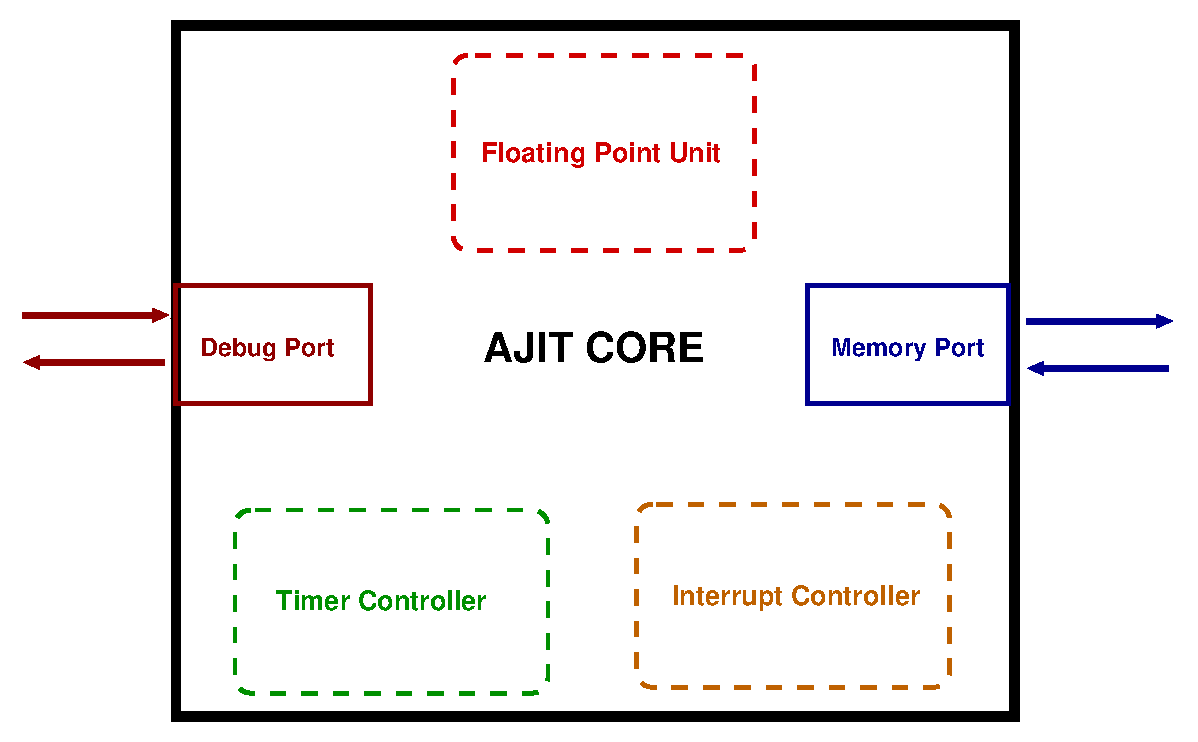
\includegraphics[scale=0.7]{eps_pdf_sources/ajit_fpga/AJIT/ajit_intro}
\caption{Overview of AJIT}
\end{figure}

\subsection{Support for AJIT}

AJIT has a functionally correct and verified C model which is used to verify new additions to the processor and user space
applications. AJIT also has a VHDL model which we incorporate into the later stages of this project and the same model later on loads
different programs ( before testing loading of an OS ) directly from the DRAM. 

\section{Introduction to the Project}

The main aim of this project is to provide an alternative to an earlier FPGA model designed around AJIT processor which had limited
on-board memory of 4MB and hence could borderline load a Linux system since the minimum memory requirement for a Linux operating system to
boot is around 4MB. The operating system thus loaded/booted had very limited kernel modules and userspace drivers to interface with hardware
elements.\\

This project is focussed at leveraging high DRAM storage capabilities and the high read and write speed of PCIe bus of the Xilinx VC709
board in order to make it capable to boot a heavily loaded embedded OS( quite possibly an RTOS ) with all the basic kernel modules and
userspace drivers to interface with hardware elements such as networking.\\

This process of booting an embedded OS on a FPGA platform is really advantageous as compared to booting OS on development boards based
around ASICs as we outline later. This project aims to integrate this FPGA system with a \verb|C++| based application to implement
a router system down the line.\\

We aim to incorporate soft core peripherals such as a Ethernet controller, USB controller etc to this FPGA system to ease the access to the
system through \verb|ssh| connections or through \verb|serial| connections. These kinds of easily integrable peripherals are expected to
make the development of custom applications really swift.\\

This project as we demonstrate later can also be used as a test-bed for HPC codecs development and testing. These peripherals can be
distributed along with the AJIT processor as part of its HPC peripheral library.


\chapter{Need for the System}


\chapter{Introduction to FPGA System}

\begin{figure}[H]
\centering
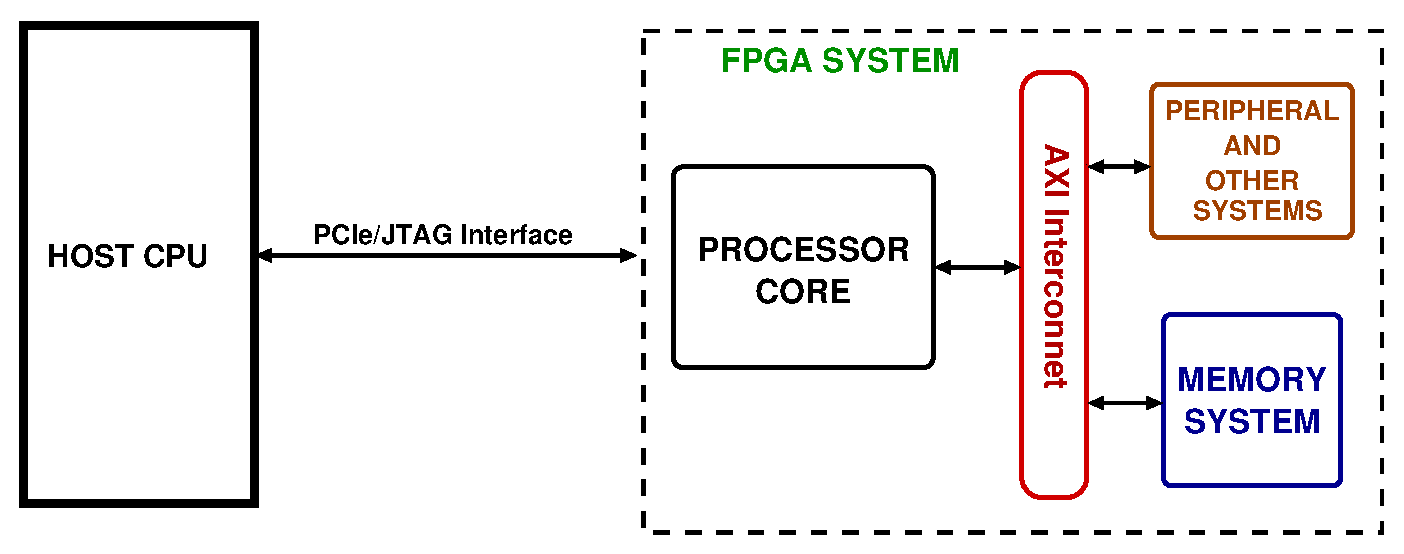
\includegraphics[width=\textwidth]{eps_pdf_sources/ajit_fpga/System_overview/fpga_system_intro}
\caption{Introduction to the FPGA System}
\end{figure}

The previous block diagram showed a telescopic view of the mentioned FPGA system. Now we expand a bit on the FPGA System block mentioned in
the previous diagram.

Here we introduce a generic interface architecture for building a system. As shown in the figure above the generic interface diagram of the
fpga model. Every subsystem including the processor core hanging from the interconnect appear just like a memory mapped peripheral to it.
This kind of architecture as explained at last in future work would provide a relatively easy extension to a Multiprocessor SMP model as
compared to a processor centric model. Some peripherals would act as AXI Slaves and some as AXI Masters depending on their functionality.
Another advantage to this architecture is that since each peripheral is memory mapped and JTAG has a direct access to the Interconnect one
can probe and read-write from-to any peripheral independent of the processor. As shown later after interfacing the PCIe to AXI we get
another possible data flow channel other than the standard UART and JTAG.  The number of peripherals that can be interfaced in this fashion
is only limited by the number of bits used for addressing on the interconnect.

\begin{figure}[H]
\centering
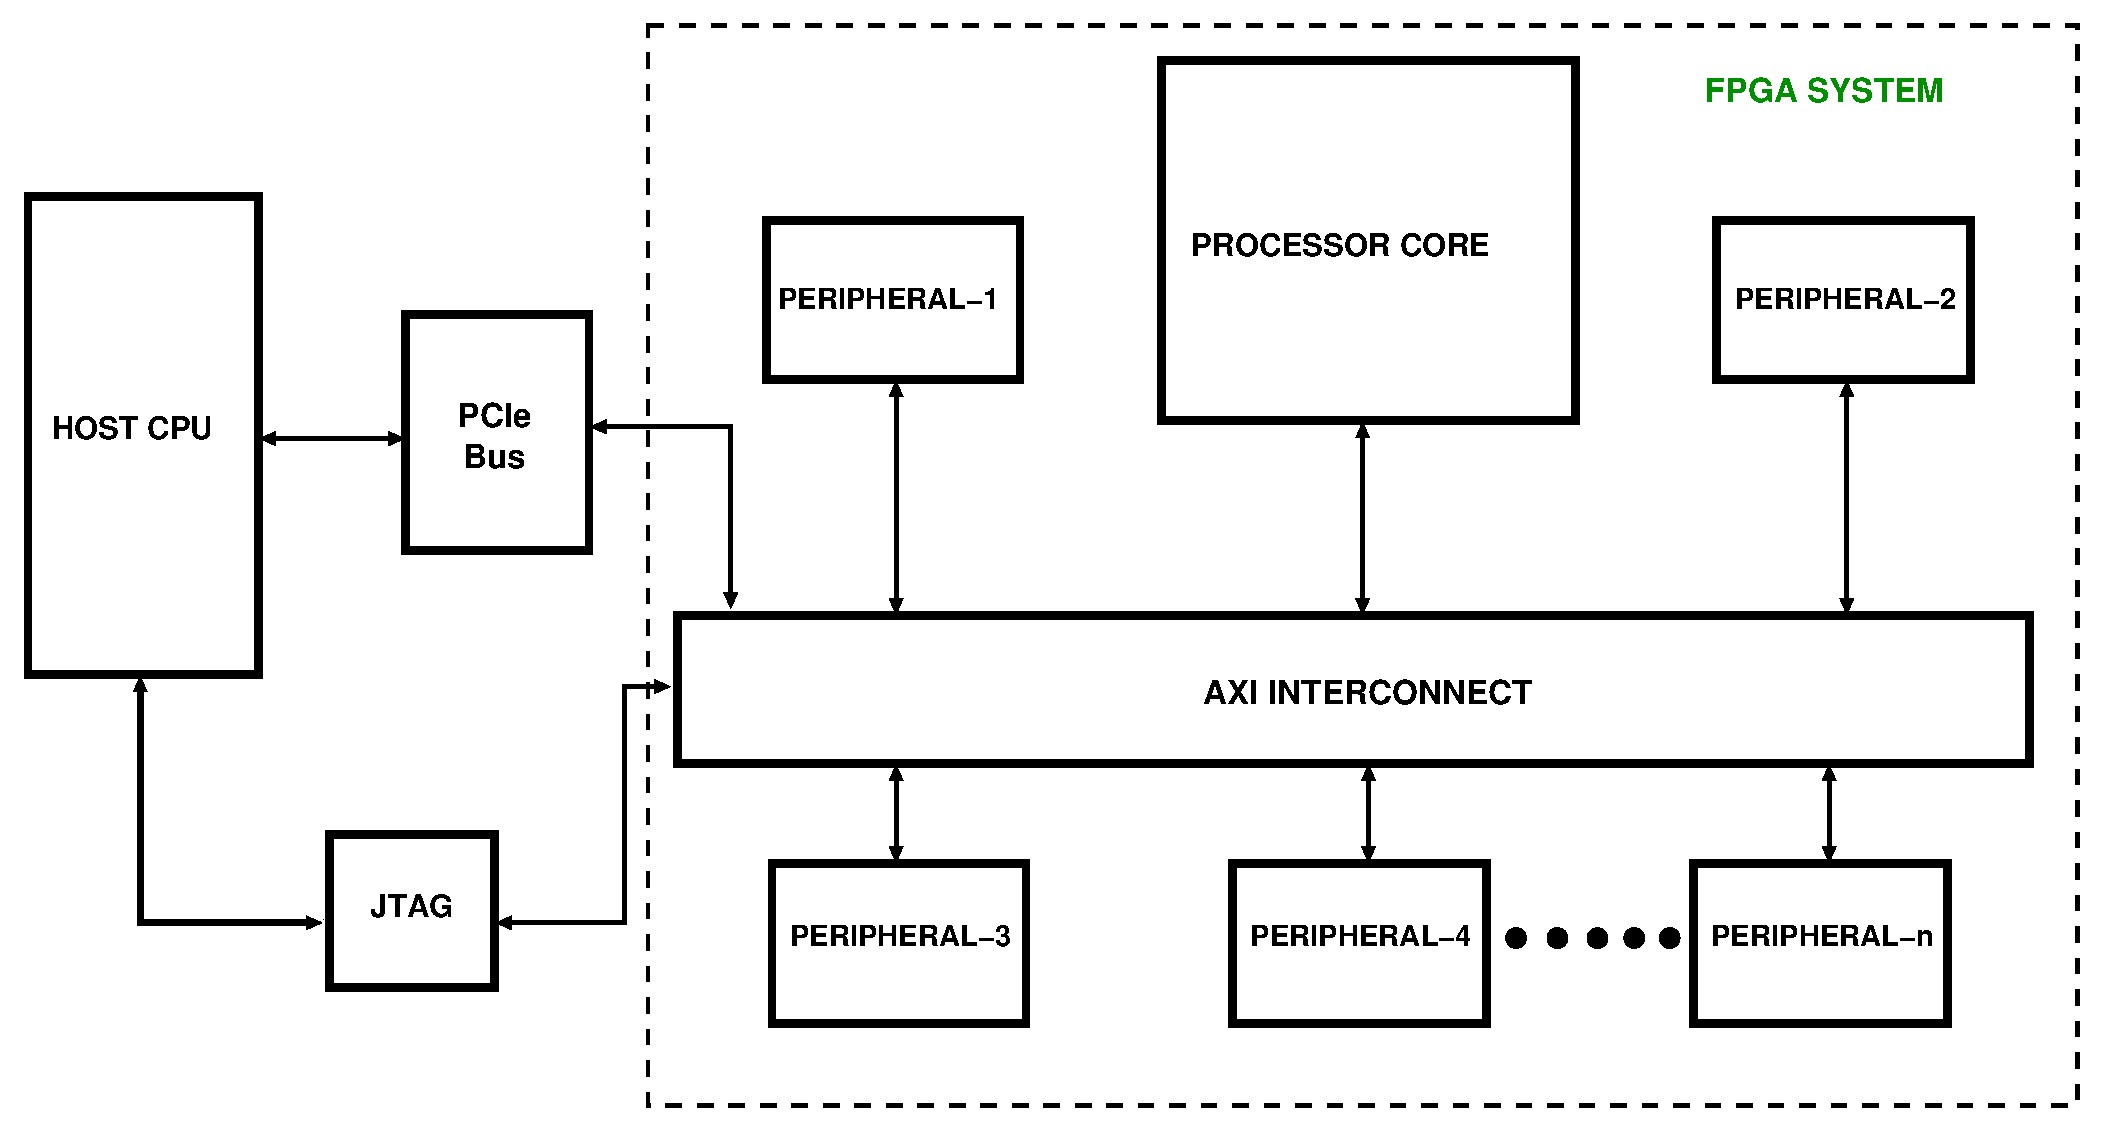
\includegraphics[width=\textwidth]{eps_pdf_sources/ajit_fpga/System_overview/fpga_system_expanded}
\caption{FPGA System Expanded}
\end{figure}


\chapter{System Level Description}

\section{Master-Slave Pairing}

The whole FPGA system development circles around this fundamental idea of Masters and slave peripherals. The slave peripheral needs to be in
the memory map of the Master peripheral so that the master can access it by making memory requests on the interconnect. The below figure
shows a 1 Master - 1 Slave configuration with an interconnect IP interfacing them. As is visible the interconnect needs both the clocks on which
the peripherals operate in order to interface them by employing dual clocking FIFOs for each AXI channel.

\begin{figure}[H]
\centering
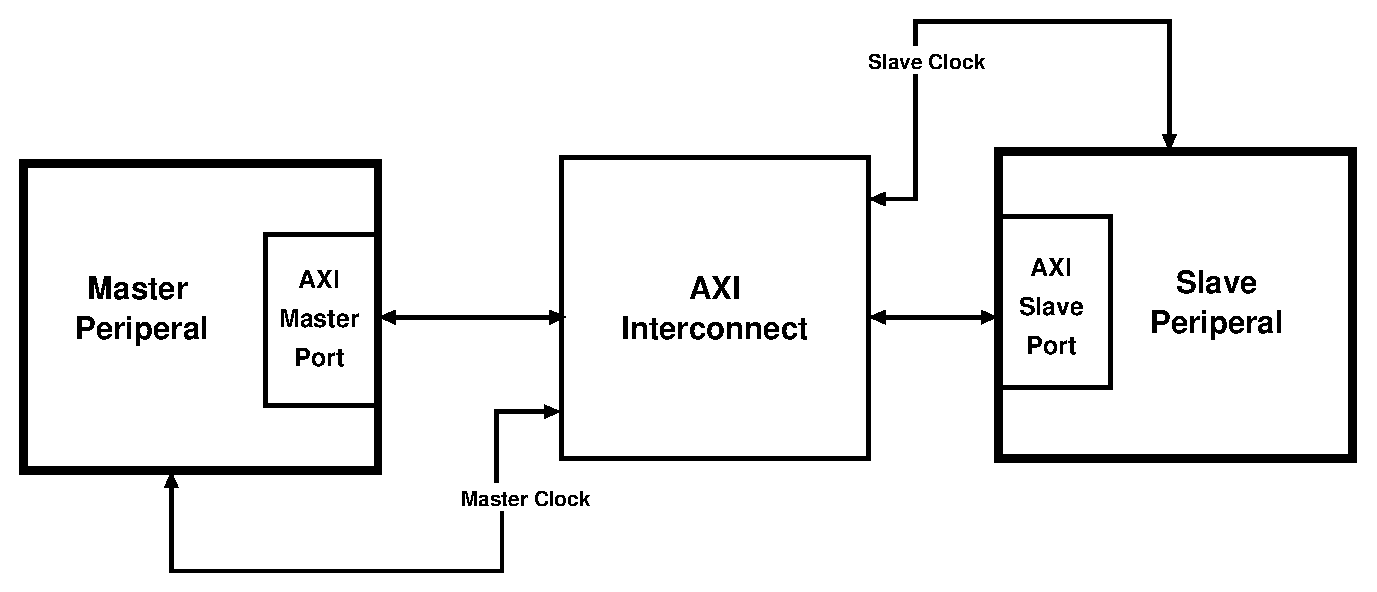
\includegraphics[width=\textwidth]{eps_pdf_sources/ajit_fpga/System_Level/One_Master_One_Slave}
\caption{1 AXI Master - 1 AXI Slave Configuration}
\end{figure}

The AXI Interconnect which bind the whole system is a NoC ( Network on Chip ) implementation of the communication subsystem and hence brings
notable improvements over conventional bus and crossbar communication architectures. Networks-on-chip improve the scalability of
systems-on-chip and the power efficiency of complex SoCs compared to other communication subsystem designs. 

\begin{figure}[H]
\centering
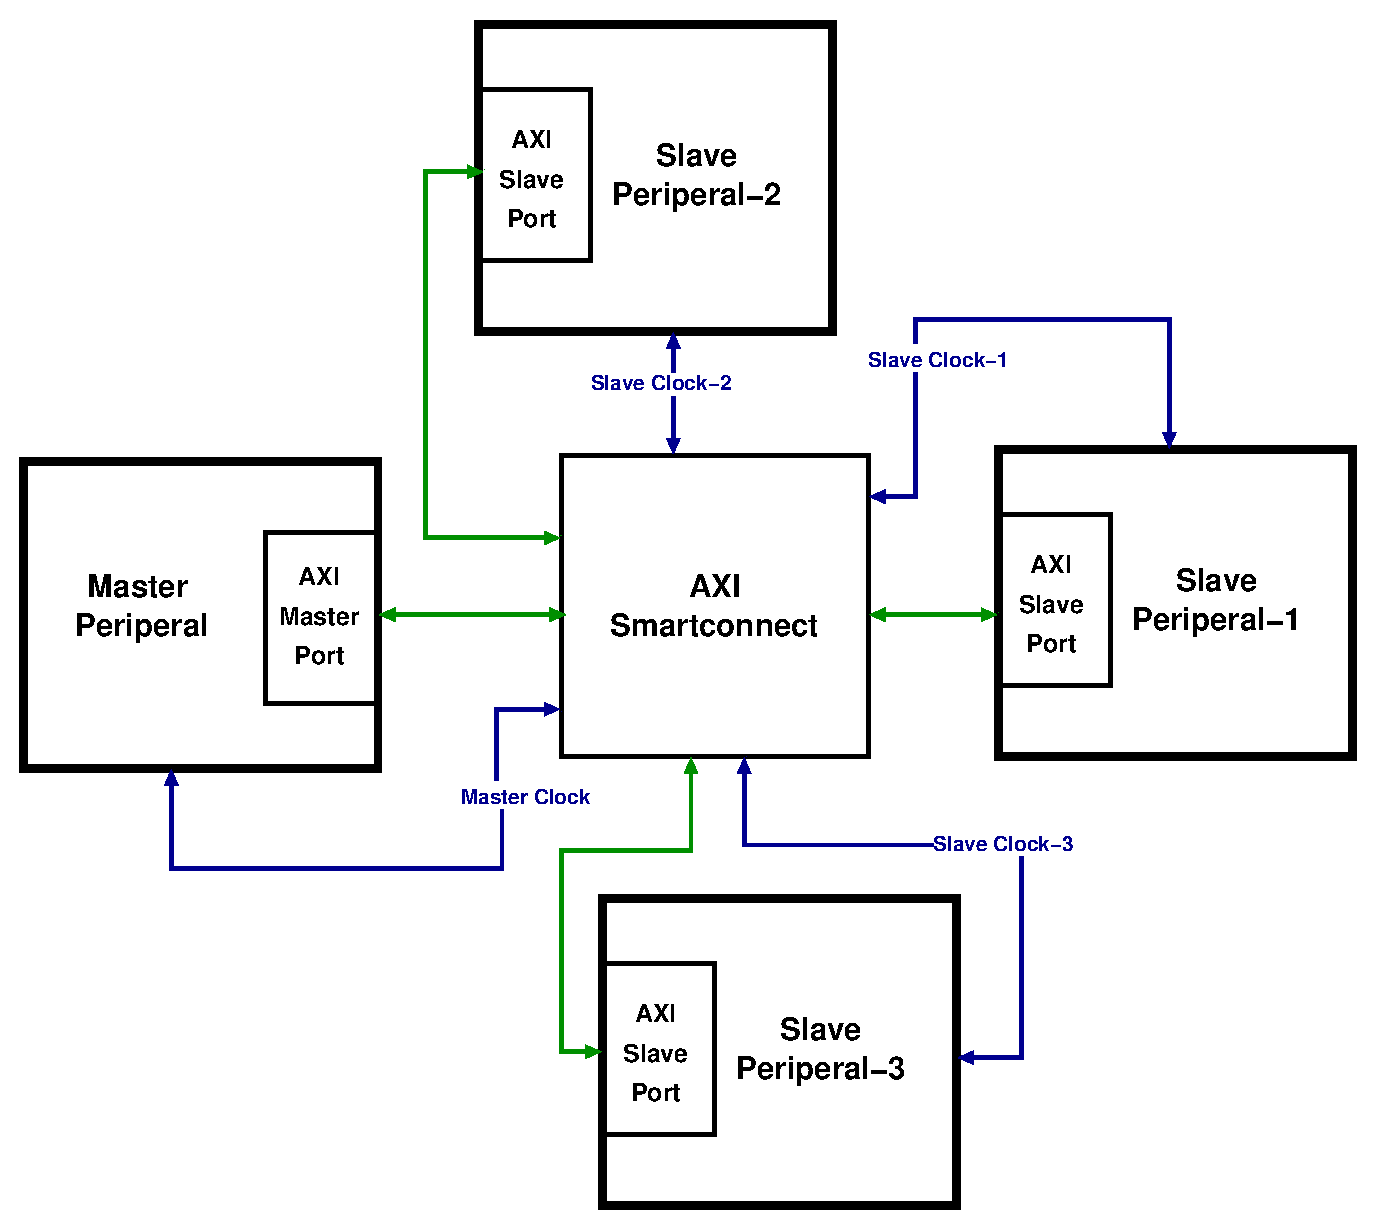
\includegraphics[width=\textwidth]{eps_pdf_sources/ajit_fpga/System_Level/One_Master_Multi_Slave}
\caption{1 AXI Master - 3 AXI Slave Configuration}
\end{figure}

\section{Dual Clocking FIFOs in Interconnects}

Dual clock FIFOs are designed for two circuits operating in different clock frequencies to communicate with each other. There is a read side
and write side where data is stored into the internal memory of the FIFO using the write side clock and then read from the internal memory
using the read side clock. AXI Smartconnect IPs from Xilinx employ dual clocking FIFOs to interface Master and slaves which have operate at
different clock frequencies for example AJIT core operates at 100MHz but the PCIe-AXI Translation IP operates at 250MHz thus we need
something like an AXI Smartconnect which can handle this interfacing situation.

\section{Memory mapped devices}

This age old approach is a regular practice on desktop, portable and embedded devices. This makes a device registers appear like a memory
location which can be manipulated with userspace applications.This makes writing to AXI peripherals through AJIT really convenient, the
reading and writing just becomes writing to the device file \verb|\dev\mem| on the AJIT Linux OS, this will initiate the appropriate memory
request from the AJIT core to the AXI interconnect through the AFB-AXI Bridge to the on board DRAM.

\section{Peripheral Control Interface}

The AXI Slave interface for each peripheral on the AXI Interconnect has some data registers and some control registers which include start
idle, and done bits. The start bit is written high after writing the data to the appropriate data registers and then the status bit i.e. the
done bit can be polled continuously until the peripheral is found to be done with the task. This is obviously a cumbersome process but works
out just fine for less number of peripherals, as the system matures we would need the peripherals to raise an interrupt to the processor
core whenever it is finished with the assigned task or if some error has occurred while execution of the task. 

\section{Processor as a peripheral} 

The AJIT processor wrapper has been designed so to have 2 AXI slave interfaces for debugging and 1 AXI Master interface for memory reads and writes
which are done indirectly through the AFB-AXI bridge as explained later. The below figure shows the wrapping done around in order to make it
in raw sense AXI interfaceable. As you can see inside the wrapper, AJIT resides in the center and right adjacent to it on the right is the
AFB-AXI Bridge which has been explained in detail later but for time being can be understood just as a bridge between the custom data bus of
AJIT i.e. AFB and the AXI interface. To the left of AJIT core are 2 64 bit FIFOs which are supposed to carry the 64 bit number sent from the
host which contains debug commands. To even further left of these FIFOs are their controllers which provide an AXI interface control of
these FIFOs to the masters on interconnect which includes the host machine(more on this later). These in combination provide AJIT
processor an interface ability to the AXI interface and makes AJIT core just another AXI Master peripheral on the AXI interconnect.\\

\begin{figure}[H]
\centering
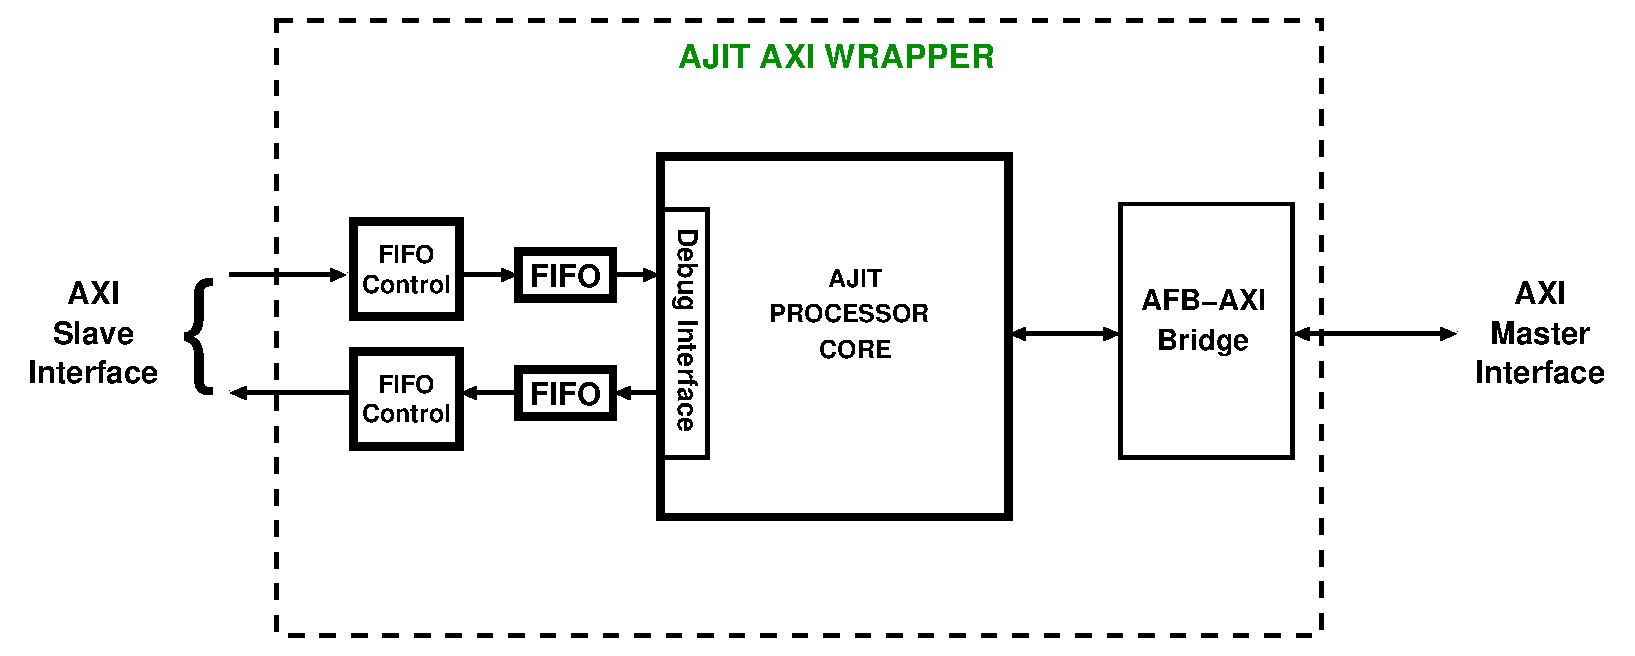
\includegraphics[scale=0.6]{eps_pdf_sources/ajit_fpga/System_Level/ajit_combined}
\caption{AJIT AXI Wrapper}
\label{ajit_combined}
\end{figure}



\chapter{Interfaces}

\section{AXI-Lite Interface}

This interface operates with 5 FIFOs with different widths namely for Write Address, Write Data, Write Response, Read Address and Read data
channel.

\begin{figure}[H]
	\centering
	\begin{subfigure}[b]{0.5\textwidth}
	\centering
	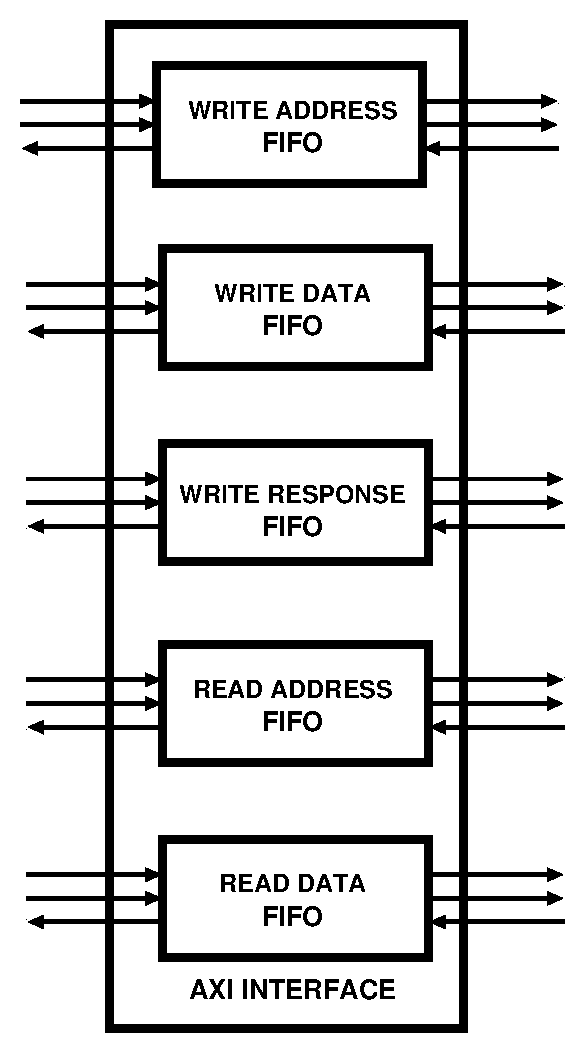
\includegraphics[width=0.7\textwidth]{eps_pdf_sources/ajit_fpga/AFB_AXI_bridge/AXI_internal_FIFOs}
	\caption{AXI-Lite FIFOs}
	\end{subfigure}
	\hfill
	\begin{subfigure}[b]{0.45\textwidth}
	\centering
	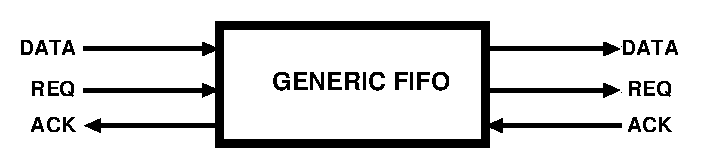
\includegraphics[width=\textwidth]{eps_pdf_sources/ajit_fpga/AFB_AXI_bridge/FIFO}
	\caption{FIFO Interface}
	\end{subfigure}
\caption{AXI-Lite Interface}
\end{figure}

\section{AFB Interface}
The master interface for the custom AFB interface is the AFB Request Interface and the corresponding slave interface is the AFB Response
Interface.

%- Need to add AFB specs table.

\subsection{AFB Response Interface}
\begin{table}[H]
\begin{tabular}{c | c | c | c}	
\hline
Port Name & Port Description & Direction & VHDL Data Type\\
\hline
AFB\_RESP\_DATA 	& Data Signal 	& in & std\_logic\_vector(32 downto 0) \\
AFB\_RESP\_READY 	& Ready Signal 	& in & std\_logic\_vector(0 downto 0)  \\
AFB\_RESP\_ACCEPT & Acceptance Signal & out & std\_logic\_vector(0 downto 0)  \\
\end{tabular}
\caption{AFB Response Interface Signals}
\end{table}

\subsection{AFB Request Interface}
\begin{table}[H]
\begin{tabular}{c | c | c | c}
\hline
Port Name & Port Description & Direction & VHDL Data Type\\
\hline
AFB\_REQ\_DATA 	 & Data Signal	     & out  & std\_logic\_vector(73 downto 0) \\
AFB\_REQ\_READY  & Ready Signal      & in   & std\_logic\_vector(0 downto 0)  \\
AFB\_REQ\_ACCEPT & Acceptance Signal & out  & std\_logic\_vector(0 downto 0)  \\
\end{tabular}
\caption{AFB Response Interface Signals}
\end{table}

\section{Req and Ack Interface Protocol}
Req and Ack protocol is a custom protocol defined by Prof.Madhav Desai wherein the environment sends out a \verb|req| signal whenever it has
data to send out and the slave responds with an \verb|ack| signal which translates to a green flag to the transaction and the data is
exchanged.  The \verb|req| and \verb|ack| signals are interchangeable and thus can be asserted by the environment or by the slave.
Figure~\ref{req_ack_protocol} shows the timing diagram for the req-ack protocol:-

\begin{figure}[H]
\centering
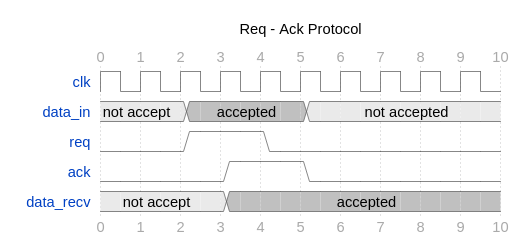
\includegraphics[width=\textwidth]{eps_pdf_sources/ajit_fpga/Interfaces/req_ack_protocol.png}
\caption{Timing diagram of Req-Ack protocol}
\label{req_ack_protocol}
\end{figure}

\section{HLS Stream Interface}
This is a trivial fifo like interface which can be generated through Vivado HLS. It uses \verb|ready| and \verb|accept| signals
instead of \verb|req| and \verb|ack|. Figure~\ref{ready_accept_protocol} shows the timing diagram for the ready-accept protocol:-

\begin{figure}[H]
\centering
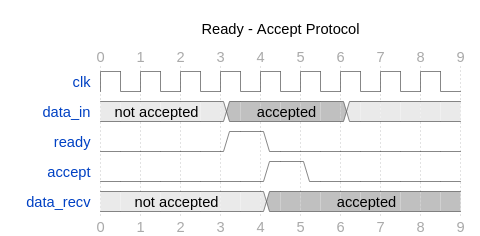
\includegraphics[width=\textwidth]{eps_pdf_sources/ajit_fpga/Interfaces/ready_accept_protocol.png}
\caption{Timing diagram of HLS stream interface}
\label{Ready-Accept protocol}
\end{figure}


\chapter{Blocks Description}

%\section{AJIT Core}

%- Need to add the ajit expanded core diagram with debug ports labelled.

%\begin{figure}[H]
%\centering
%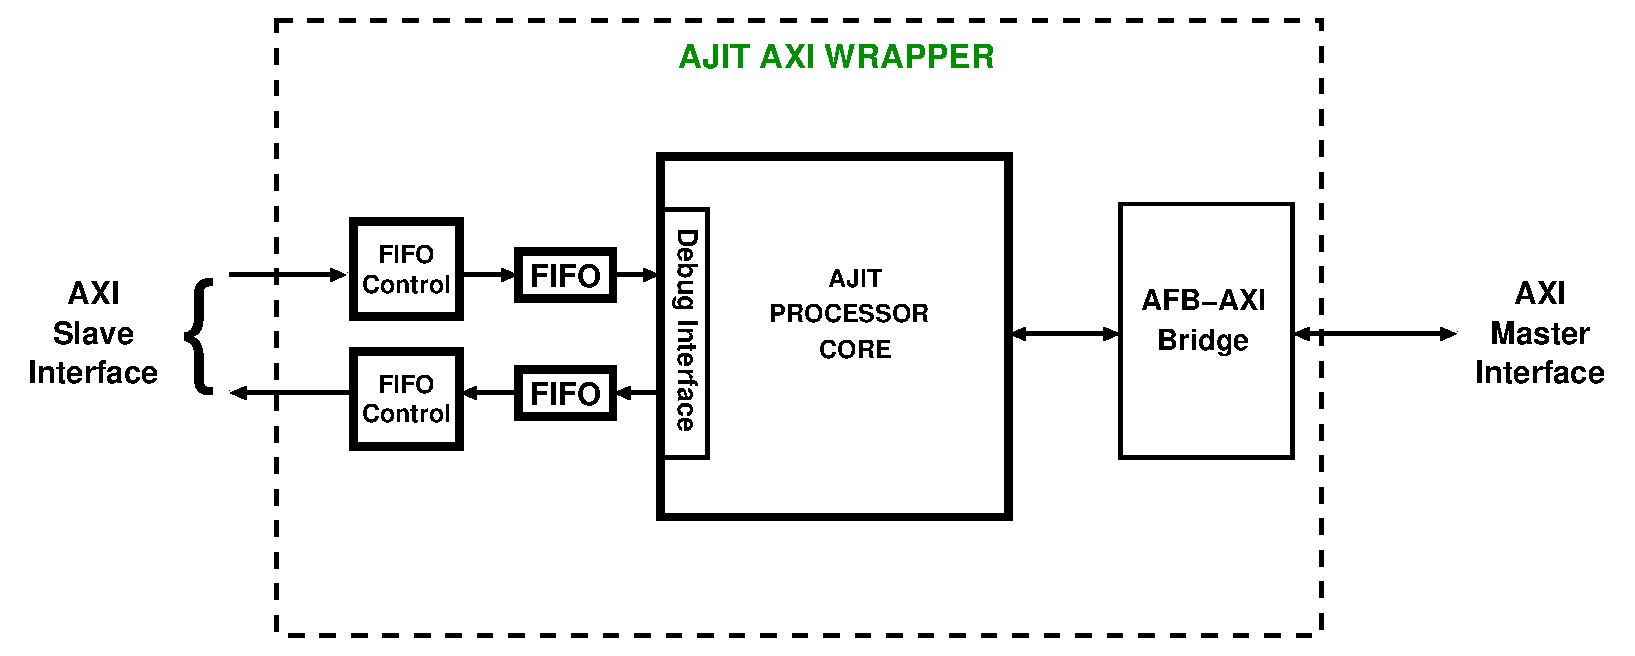
\includegraphics[scale=0.6]{eps_pdf_sources/ajit_fpga/System_Level/ajit_combined}
%\caption{AJIT AXI Wrapper}
%\label{ajit_combined}
%\end{figure}

\section{DRAM Controller}

\subsection{Need for a DRAM interface}

In the previous iteration of OS booting on AJIT processor the OS utilized the block RAM of the processor which was of size 4 MB
and thus took awhile to boot and only a small scale OS without much driver support(like Network drivers) could be booted, thus a need for a
larger DRAM support.  Here we head out to utilize the onboard DRAM of the VC709 board based on the ideas of our generic peripheral
interface discussed before.

\subsection{Our implementation}

The figure~\ref{DRAM Controller integrated flow} below shows our DRAM interface implementation as part of a generic AXI peripheral system.
DRAM interfaces with the AXI interconnect with the aid of a Memory Controller specifically employed for DRAMs. Memory controller was
generated using the MIG (Memory Interface Generator) utility of Vivado 2017.1. 

The support for DRAM size here goes up to 4 GB per slot and since VC709 has two slots we can have a combined support up to 8GB RAM.

\begin{figure}[H]
\centering
\includegraphics[width=\textwidth]{eps_pdf_sources/ajit_fpga/DRAM_without_PCIe/DRAM_without_PCIe}
\caption{DRAM Controller integrated flow}
\label{DRAM Controller integrated flow}
\end{figure}

\subsection{MIG Vs EMC Core}

The two cores provided in Vivado are for different types of memory. The following information can be found in the respective user guides
which summarise their use cases:

\begin{table}[H]
\centering
\begin{tabular}{c | c}
\hline
Core & Memory Support \\
\hline
 MIG & DDR2, DDR3, QDR-II, RLDRAM \\
 EMC & SRAM, ZBT, and other similar SRAM like interfaces \\
\end{tabular}
\caption{Comparison of Memory Cores}
\end{table}

\subsection{Testing of Interface}

We tested the interface using the XSCT command line utility which employs the JTAG interface and gives a direct access to all AXI
peripherals. Later on we also tested this with a PCI express interface from the Host CPU using the pcimem utility.

\section{PCIe-AXI IP}

\subsection{Need for a PCIe interface}

In the previous iteration of OS booting on AJIT processor the OS utilized the block RAM of the processor which was of size 4 MB
and the size of the kernel was just 2 MB and now as we increase the RAM size to accommodate a heavy duty OS we need a faster way to write
the image to the storage instead of JTAG and we are just in luck since VC709 has a PCIe interface and can be plugged directly into the PCIe
slot of the host CPU motherboard.  Right now we lack a flash interface in our system which would have allowed us to have a nonvolatile
memory block which would not require to be written at every power on-off cycle of the board. Here we utilize the PCIe interface of the
VC709 board.

\subsection{Basics of PCIe interface}

Before diving into the implementation details we need to revisit some essential basics of PCI express peripherals that would prove to be
useful here.  On a \textbf{Linux} machine one can type \verb|lspci -vv| in the console and get a detailed output of the PCIe devices
connected to the machine. Its a long list so I will explain with the example of the Xilinx's VC709 board. As can be seen from
listing~\ref{lst:lspci} the \verb|lspci| log gives out the details about the connected VC709 board's pci interface. Table~\ref{lspci
parameters} explains the relevant parameters in the \verb|lspci -vv| log.

\singlespacing
\scriptsize{
\begin{lstlisting}[language=bash, caption=lspci log,label={lst:lspci}, emph={Region, lspci, vv, 0a:00\.0}]
$ lspci -vv
...
...
0a:00.0 Memory controller: Xilinx Corporation Device 7038 
        Subsystem: Xilinx Corporation Device 0007 
        Physical Slot: 3 
        Control: I/O+ Mem+ BusMaster- SpecCycle- MemWINV- VGASnoop- ParErr+ Steppi......
        Status: Cap+ 66MHz- UDF- FastB2B- ParErr- DEVSEL=fast >TAbort- <TAbort- <M......
        Interrupt: pin A routed to IRQ 16 
        Region 0: Memory at f0000000 (32-bit, non-prefetchable) [size=128M] 
        Region 1: Memory at e8000000 (32-bit, non-prefetchable) [size=128M] 
        Region 2: Memory at e0000000 (32-bit, non-prefetchable) [size=128M] 
        Region 3: Memory at d8000000 (32-bit, non-prefetchable) [size=128M] 
        Region 4: Memory at d0000000 (32-bit, non-prefetchable) [size=128M] 
        Region 5: Memory at c8000000 (32-bit, non-prefetchable) [size=128M] 
        Capabilities: <access denied> 
        Kernel modules: riffa
\end{lstlisting}
}

\begin{table}[H]
\centering
\begin{tabular}{c | c}
\hline
Parameter & Value\\
\hline
PCIe slot name & 0a:00.0 \\
Class & Memory Controller\\
Device id & 7038 \\
Physical slot & 3 \\
ProgIf & Region \textit{X} \\
Kernel modules option & riffa
\end{tabular}
\caption{lspci parameter description}
\label{lspci parameters}
\end{table}

\normalsize
\doublespacing
\begin{flushleft}
\textit{X is an integer from 0 to 5\\}
\textit{ProgIf : Programming Interface\\}
\textit{Kernel Modules: Kernel module reporting that it is capable of handling the device (optional, Linux only) for example here riffa\\}
\textit{Device id : This comes in handy when there are mulitple boards connected to the host}
\end{flushleft}

\subsection{BARs and address translation}

Whenever reading or writing we proceed with a method of providing a base address and the offset along with it which would amount to the
actual address.  We operate here with what is knows as BAR( Base Address Register ), it is the register which would hold the base/start
address of your Memory block which is DRAM here. One can make multiple BARs with different base addresses to access different parts of the
memory. Each BAR is set with a base address and an address range which it can access. Each bar created by the user gives rise to a new
resource file in the /sys/ directory of the host machine which as explained later in driver development can be used to access the respective
memory locations. The listing~\ref{lst:resource} shows the created resource files inside the \verb|/sys/bus/pci/devices/0000:0a:00.0/|
directory on the host machine in this case.

\singlespacing
\scriptsize{
\begin{lstlisting}[language=bash, caption=Resource files, label={lst:resource}, emph={root, irq, resource0, resource1, resource2, resource3, resource4, resource5}]
$ ä\textbf{ls -l /sys/bus/pci/devices/0000\:0a\:00.0/}ä
...
...
-r--r--r-- 1 root root      4096 Jun 18 15:30 irq
-rw------- 1 root root 134217728 Jun 18 16:17 resource0
-rw------- 1 root root 134217728 Jun 18 16:17 resource1
-rw------- 1 root root 134217728 Jun 18 16:17 resource2
-rw------- 1 root root 134217728 Jun 18 16:17 resource3
-rw------- 1 root root 134217728 Jun 18 16:17 resource4
-rw------- 1 root root 134217728 Jun 18 16:17 resource5
...
...
\end{lstlisting}
}
\normalsize
\doublespacing

\begin{flushleft}
134217728 \textit{bytes} = 128MB\\
\end{flushleft}

The \verb|irq| file provides memory mapped support for the interrupts recieved from the PCIe-AXI Translation IP on the FPGA system.
This could be later on used as an alternate to the current polling stratgey of the custom PCIe driver as explained later.\\
The figure~\ref{PCIe flow} shows our PCIe-AXI interface implementation as part of a generic AXI peripheral system.  

\begin{figure}[H]
\centering
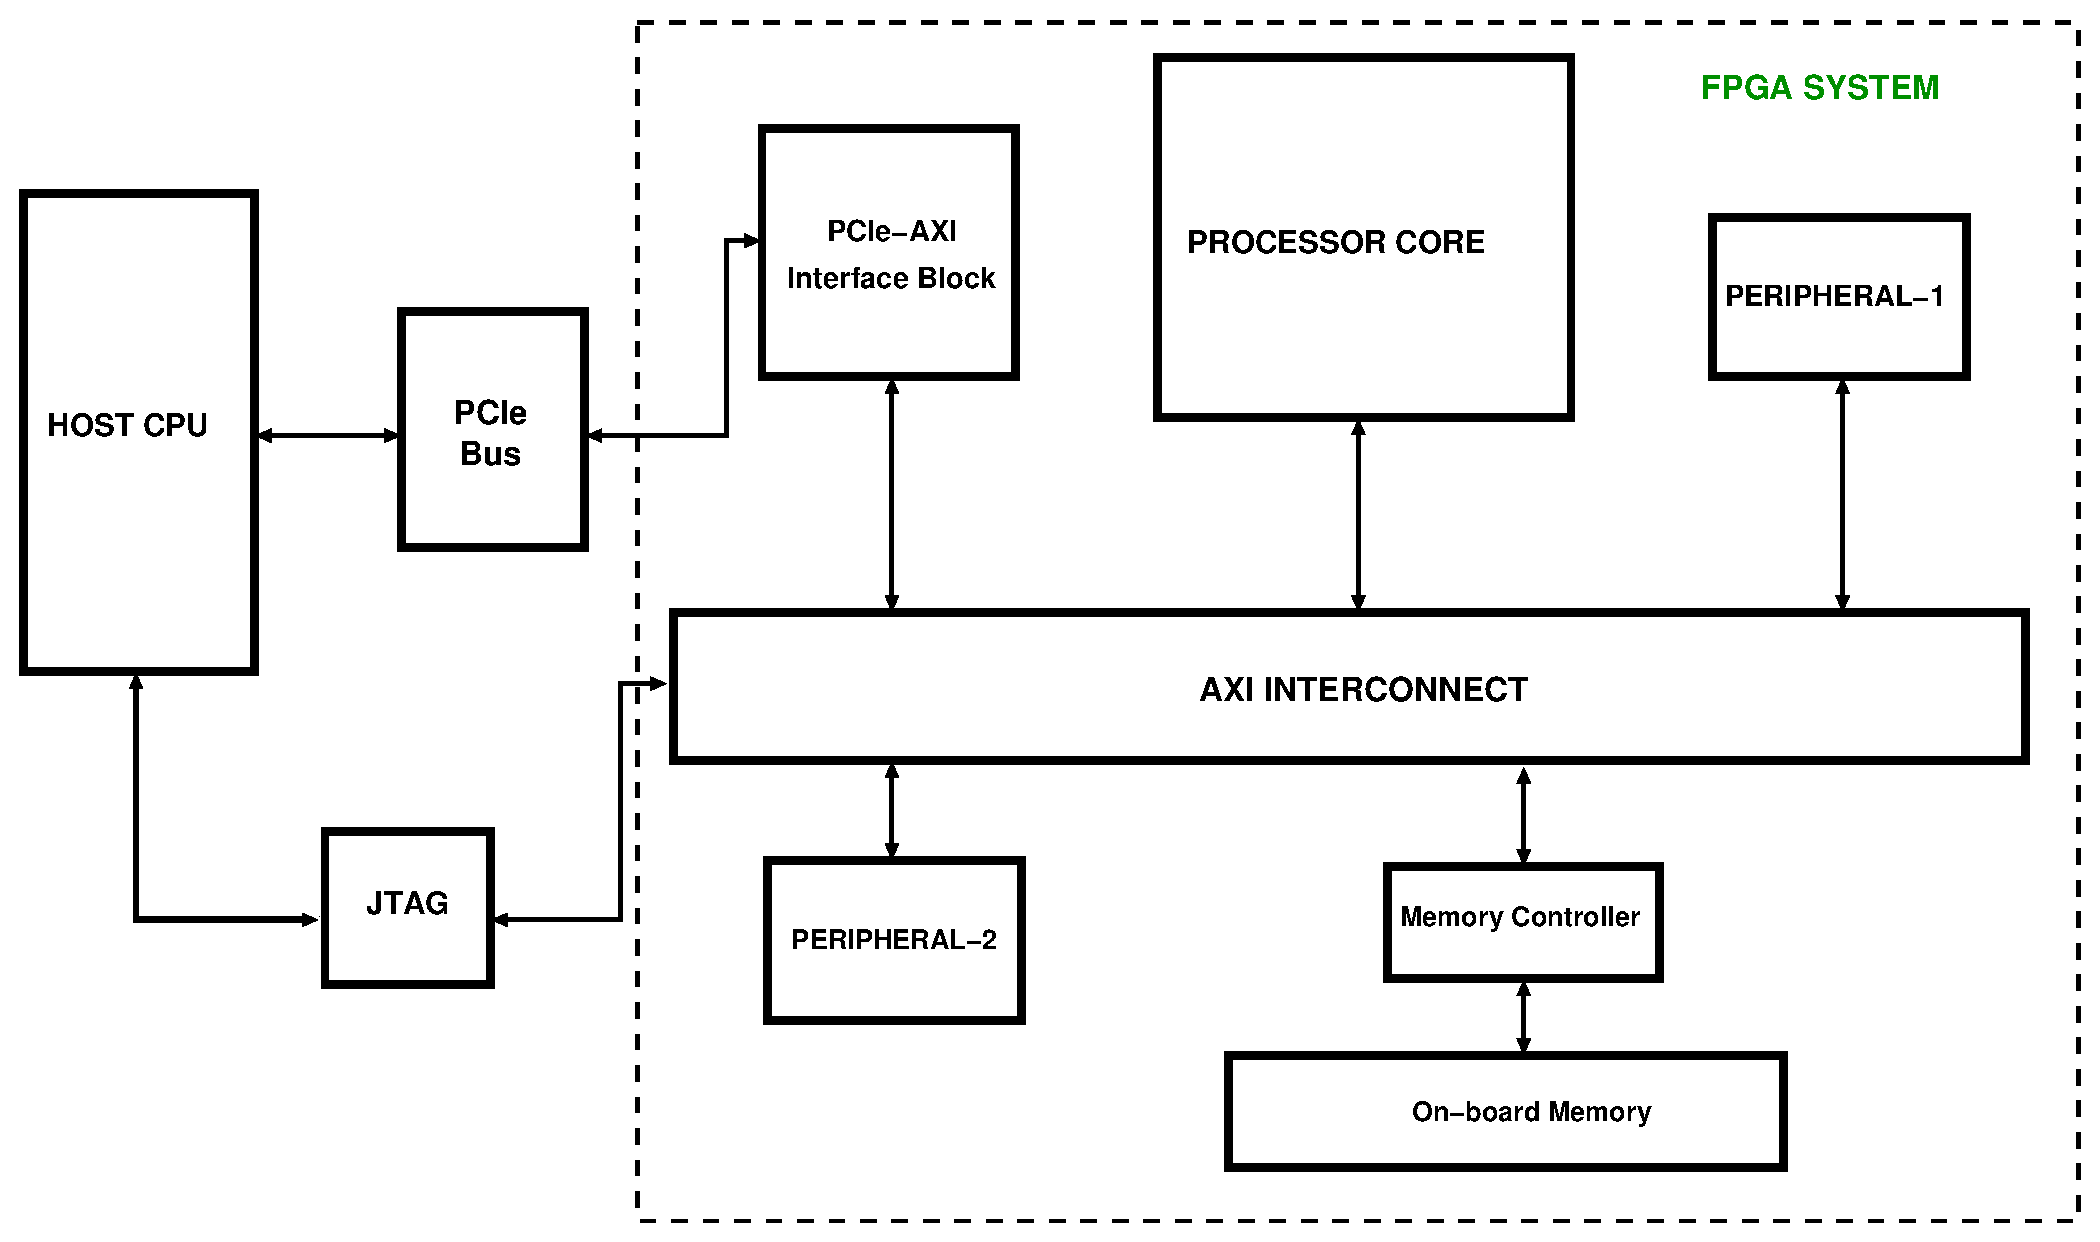
\includegraphics[width=\textwidth]{eps_pdf_sources/ajit_fpga/DRAM_with_PCIe/DRAM_with_PCIe}
\caption{PCIe-AXI interface and DRAM info flow}
\label{PCIe flow}
\end{figure}

\subsection{Testing}

We tested this with a PCI express interface from the Host CPU using the pcimem utility. Later on we developed a C driver for creating an
API interface which provides helper functions for sending and receiving information through the PCIe-AXI interface to the FPGA model.

\section{AFB-AXI Bridge}

\subsection{Need for a Custom IP for AFB-AXI Interface}

AFB(AJIT FIFO Bus) is an in-house term coined to represent the data bus of AJIT which allows it to talk to other AXI peripherals. AFB is not
directly AXI compatible and thus needs a bridge, we developed it from scratch in Verilog keeping in mind the provided AFB specifications.

\subsection{Our implementation}

We generated a custom IP bridge by writing a Verilog file and then packaging an IP through Vivado's IP Manager to make it available in the
user repository in Vivado IP repository. The bridge supports AXI-Lite on one side and AFB on the other. As can be seen in
figure~\ref{AFB-AXI bridge} the input port on the left directly interfaces with the AJIT core and then passes on the input AJIT request to
the AFB parser block which then splits the request according to the AFB specs as mentioned before and packages it as AXI Master packets and
forwards the packets to the corresponding AXI bridge's FIFOs i.e. write address, write data and read address. It also reads the the response
FIFO and the read data FIFO and packages the AXI FIFO's data back into the AFB response format and sends it back to AJIT core.

\begin{figure}[H]
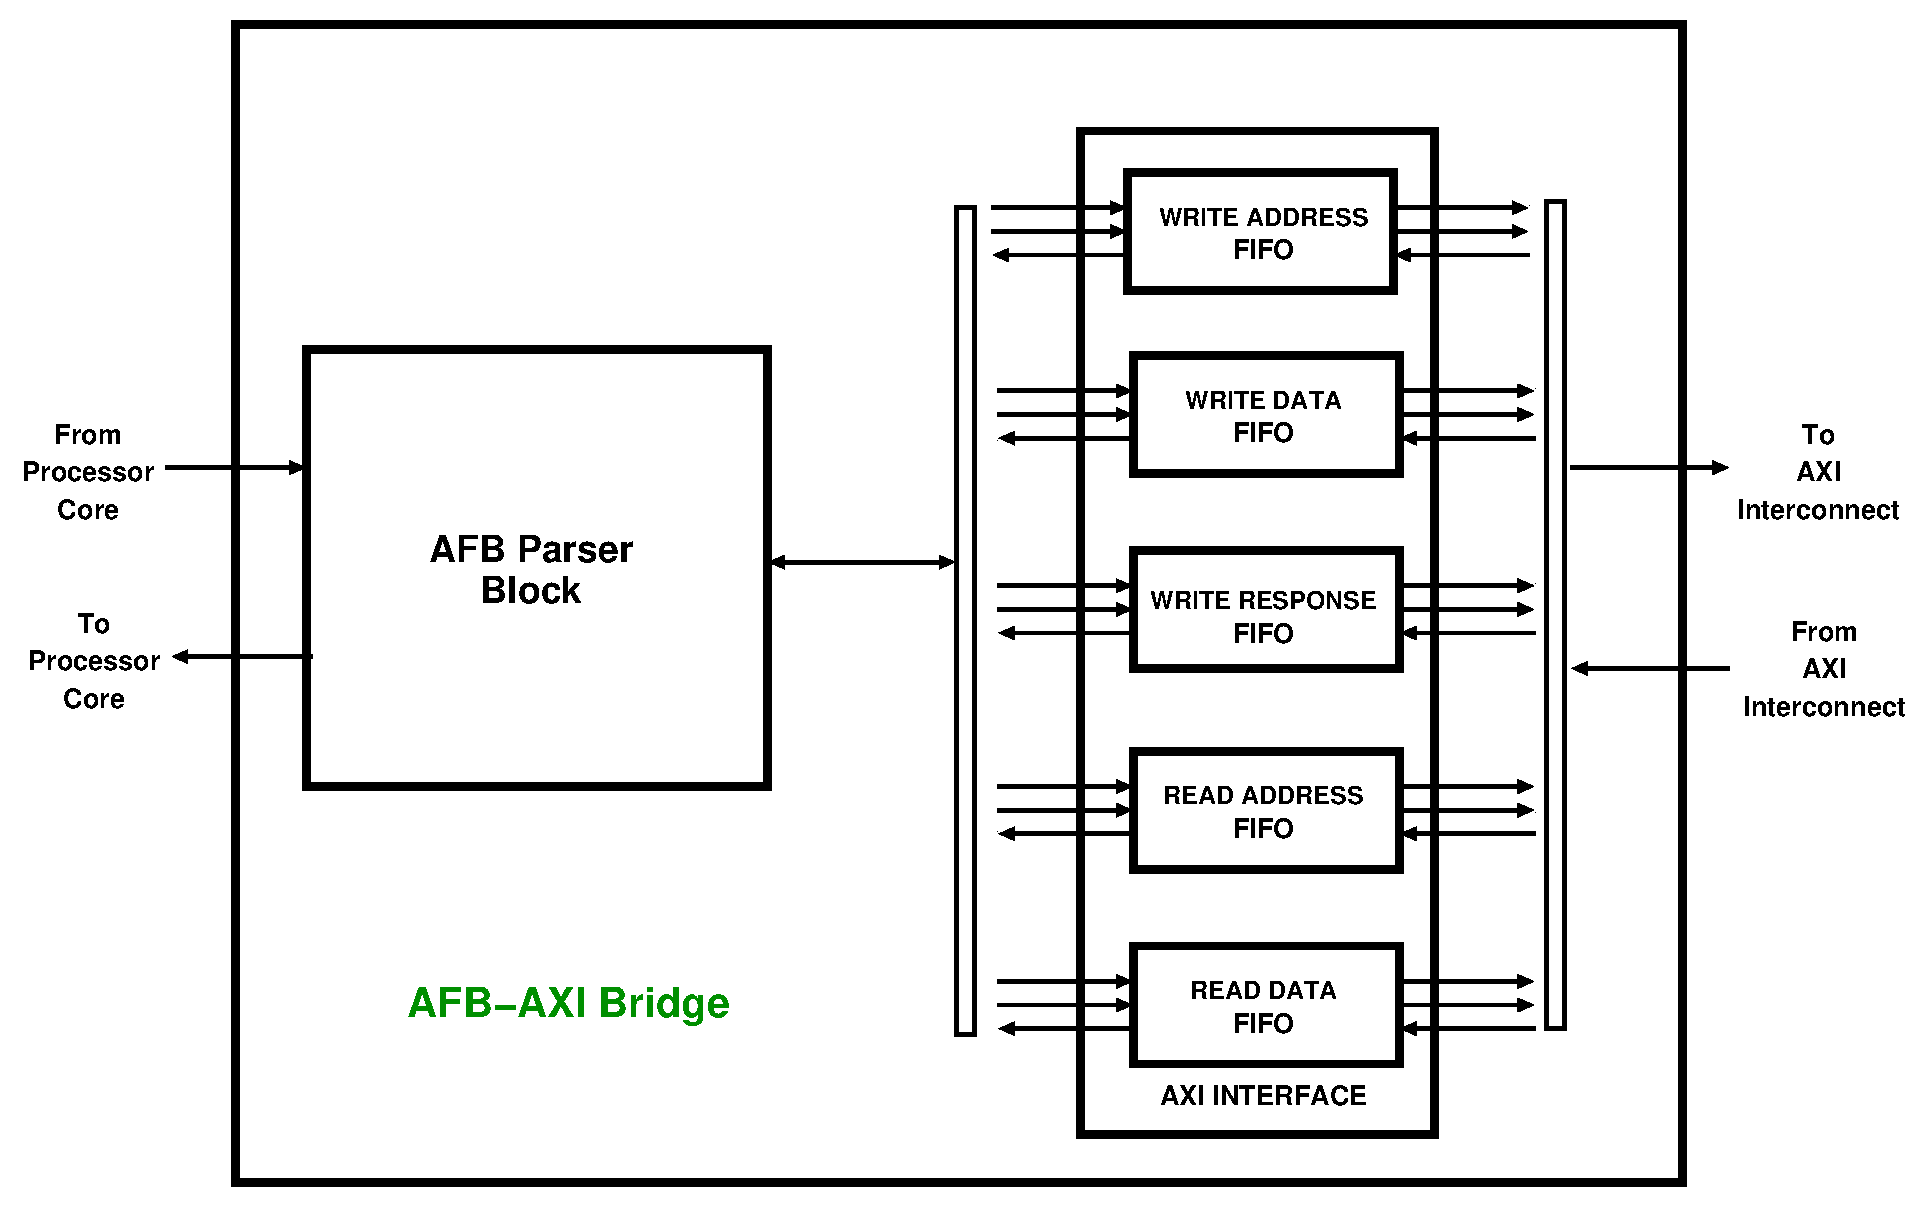
\includegraphics[width=\textwidth]{eps_pdf_sources/ajit_fpga/AFB_AXI_bridge/AFB_AXI_bridge_expanded}
\caption{AFB-AXI Bridge}
\label{AFB-AXI bridge}
\end{figure}

\subsection{Full Flow}

The figure below shows the full flow model integrated with the AFB-AXI bridge.

\begin{figure}[H]
\centering
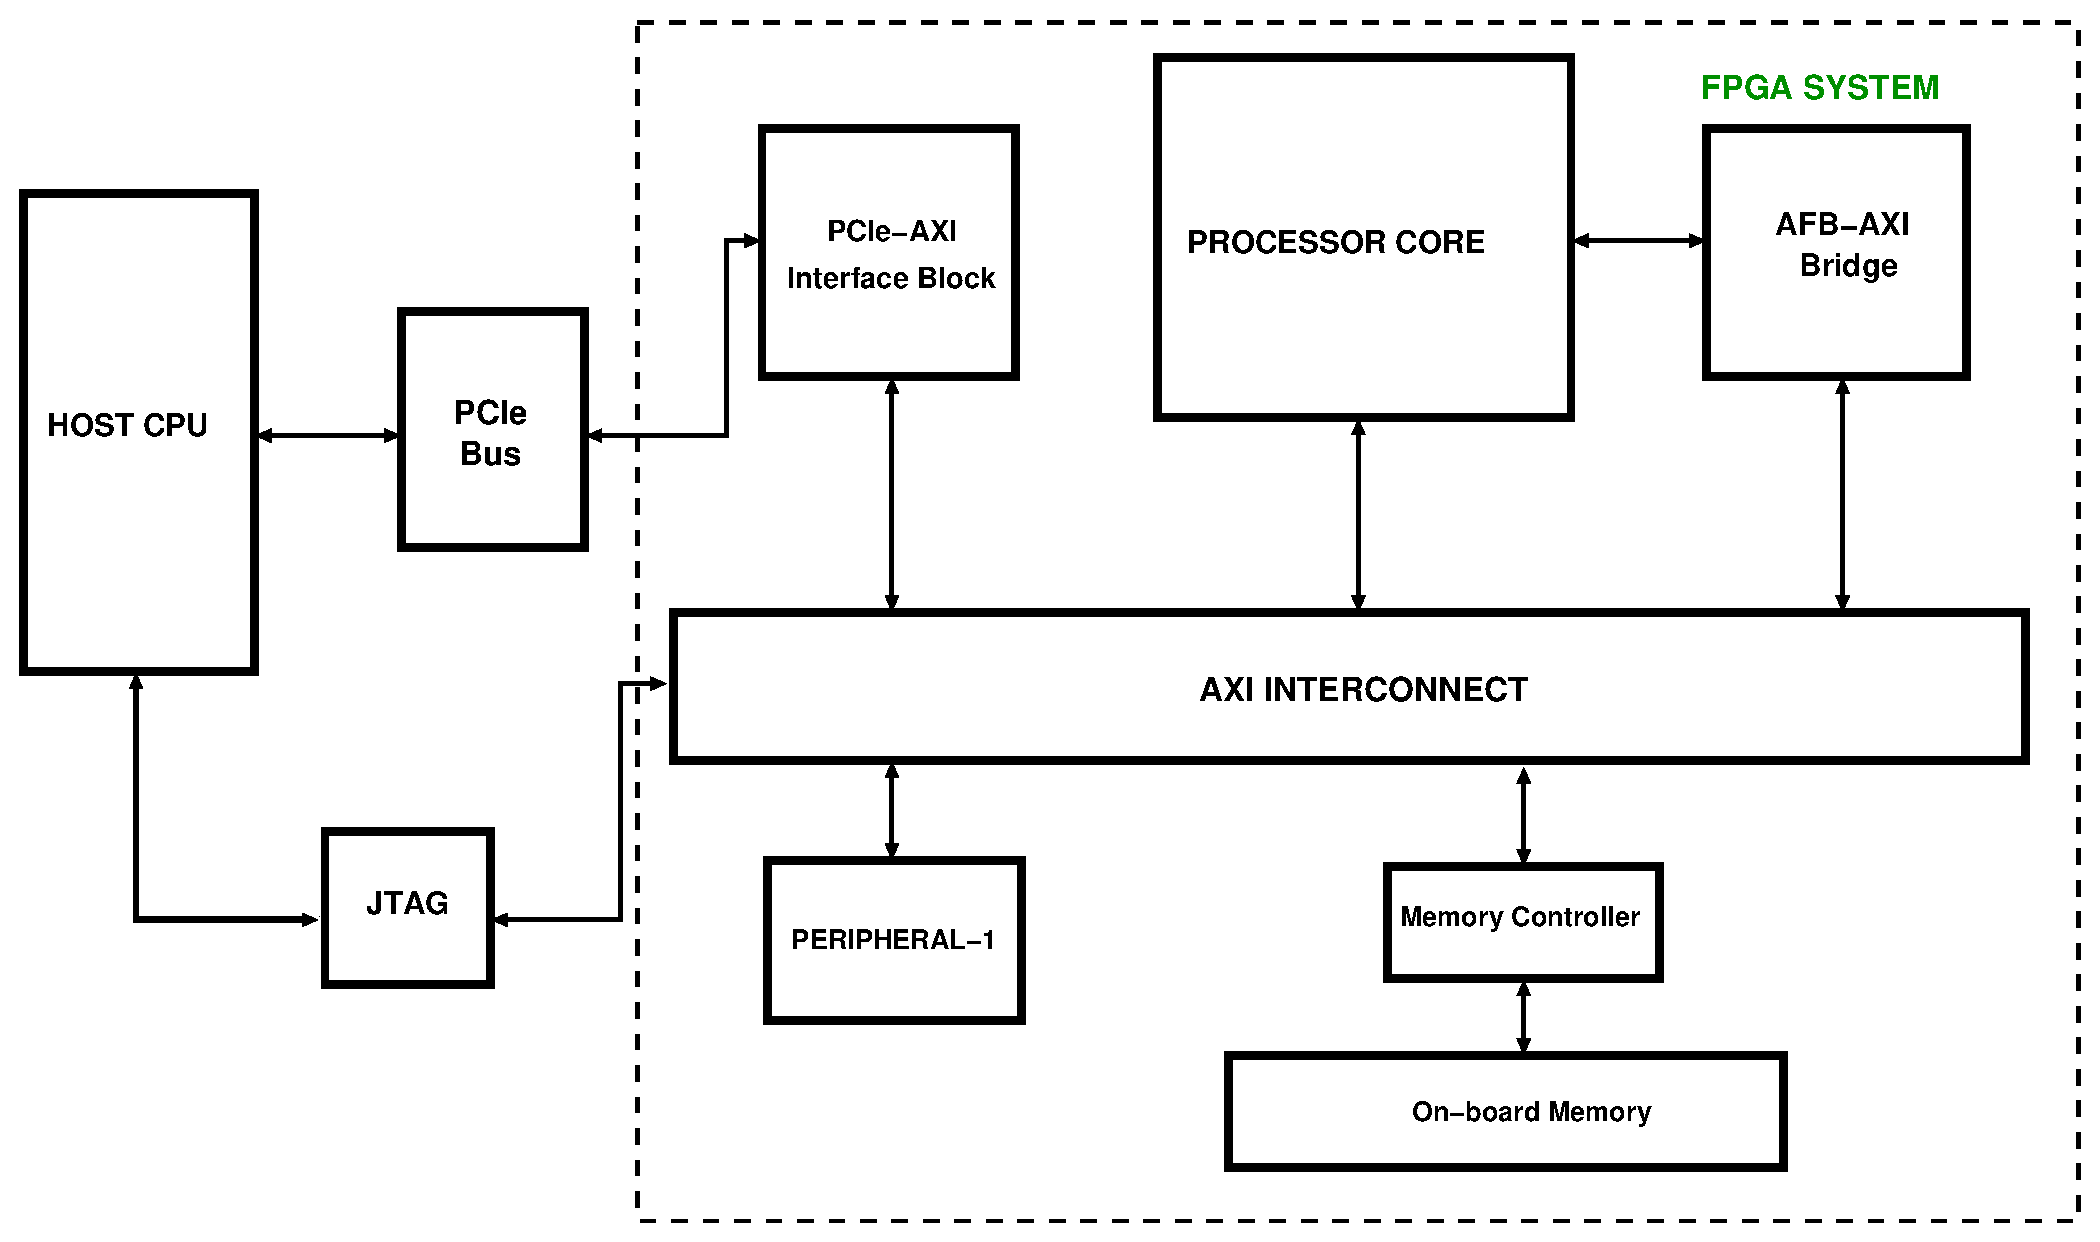
\includegraphics[width=\textwidth]{eps_pdf_sources/ajit_fpga/AFB_AXI_bridge/AFB_AXI_bridge_integrated}
\caption{Flow with AFB-AXI Bridge}
\end{figure}

\subsection{Testing of Interface}

We conducted manual memory read-write tests on the interface using the XSCT command line utility which employs the JTAG interface and gives
a direct access to all AXI peripherals. Later on we also tested this with a PCI express interface from the Host CPU using the pcimem
utility.

\section{FIFOs }

Figure~\ref{fifo} shows the generic fifo interface generated by AHIR which has been used at almost all interfaces in the FPGA system design.
The AXI side interface \verb|hls_stream| though uses a similar FIFO but with READY and ACCEPT signals instead of REQ and ACK. The timing
diagram for the same has been shown in figure.%~\ref{}.

\begin{figure}[H]
\centering
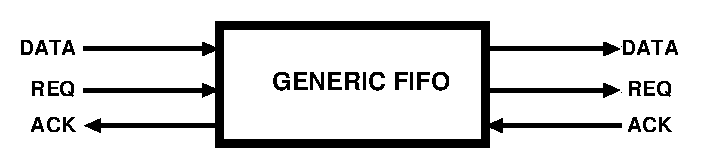
\includegraphics[width=\textwidth]{eps_pdf_sources/ajit_fpga/AFB_AXI_bridge/FIFO}
\caption{Generic FIFO Interface}
\label{fifo}
\end{figure}

\section{FIFO Controllers}

\subsection{Need for a Memory Mapped FIFO}

The Debug interface to the processor requires two 64-bit FIFOs compatible with the generic AXI peripheral interface. Here by compatibility
we mean they need to have a Slave AXI interface in order to establish a bidirectional data flow through the PCIe-AXI interface.

The problem is solved by dividing it into two parts and both of them handling simpler generic tasks. The first block provides the Slave AXI
interface as an input and a control interface on the output side to the other block which acts as a data FIFO. A similar block is created to
perform the reverse operation as well.

\subsection{Our implementation}

%\onehalfspacing
We employ \textbf{Vivado HLS}(High Level Synthesis) to generate the FIFO controllers. This enables us to write short code snippets as shown
in listing~\ref{lst:fifo controller hls} to generate the Slave AXI data interface and control signals for the FIFO controller which would
read AJIT's response from the FIFO and write it in it's slave register. The cpp template \verb|hls_stream| generates the FIFO compatible
interface so that the controller can enque and deque the debug FIFO.  Table~\ref{pragma description} provides explanation for the important
\verb|pragma| statements.

\scriptsize
\singlespacing
\begin{lstlisting}[language=C++, caption=FIFO Controller HLS, label={lst:fifo controller hls}]
void fifo_to_axi_slave (ap_uint<32> data_out, ..., hls::stream<ap_uint<32> > &in_fifo) {
    #pragma HLS INTERFACE s_axilite port=return
    #pragma HLS INTERFACE s_axilite port=data_out
    #pragma HLS INTERFACE s_axilite port=data_valid
    if (!in_fifo.empty ()) {
        data_out   = in_fifo.read ();
        data_valid = true;
    }
    else {
        data_valid = false;
    }
}
\end{lstlisting}

\normalsize
\doublespacing

\begin{table}[H]
%\centering
\begin{tabular}{| l | l |}
\hline
Pragma Statement & Description\\
\hline
HLS INTERFACE s\_axilite port return & Generates the control signals (start, done etc.)\\
HLS INTERFACE s\_axilite port data\_out & Memory mapped register for read data\\
HLS INTERFACE s\_axilite port data\_valid & Memory mapped register for data valid signal\\
\hline
\end{tabular}
\caption{Pragma Statement Description}
\label{pragma description}
\end{table}

\subsection{Full Flow}

The figure~\ref{full system} shows our complete FPGA implementation as a generic AXI peripheral system. AJIT core interfaces with the DRAM controller
indirectly through the AFB-AXI bridge which translates its requests to the AXI format, AJIT interfaces to the host machine through the debug
interface which is also AXI compatible and is controlled by the host through the PCI-AXI translation bridge which is used to translate PCIe requests to AXI
requests but the interesting thing to note is that it can also be controlled by on-board master peripherals for example the processor. The
figure~\ref{full system with flow} shows the crucial data flows in the FPGA system.

\begin{figure}[H]
\centering
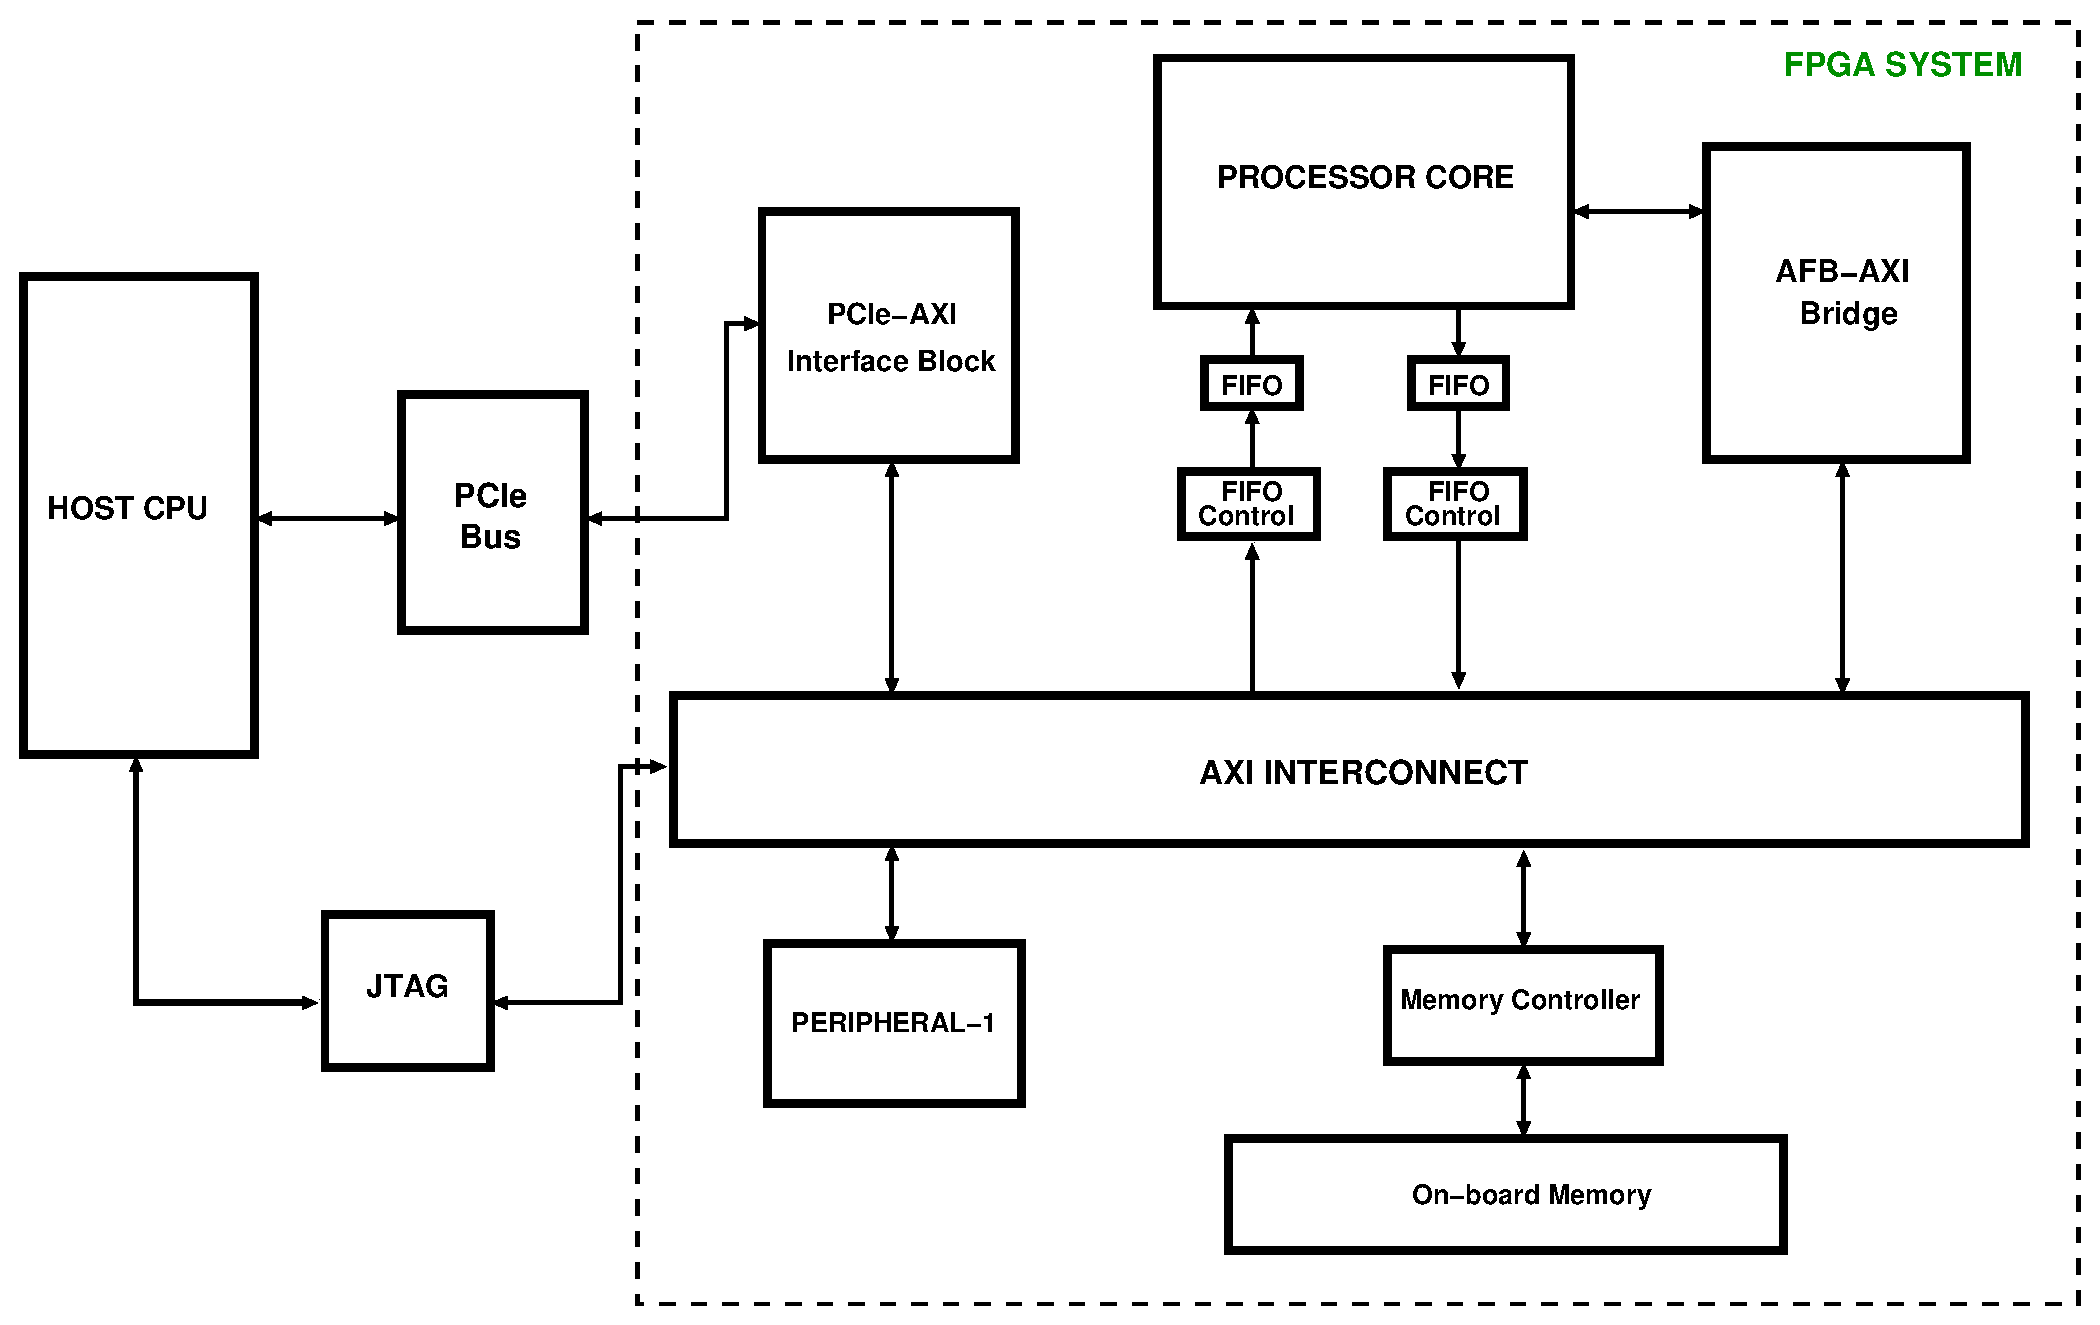
\includegraphics[width=\textwidth]{eps_pdf_sources/ajit_fpga/Full_System/Full_system}
\caption{Complete FPGA system}
\label{full system}
\end{figure}

\begin{figure}[H]
\centering
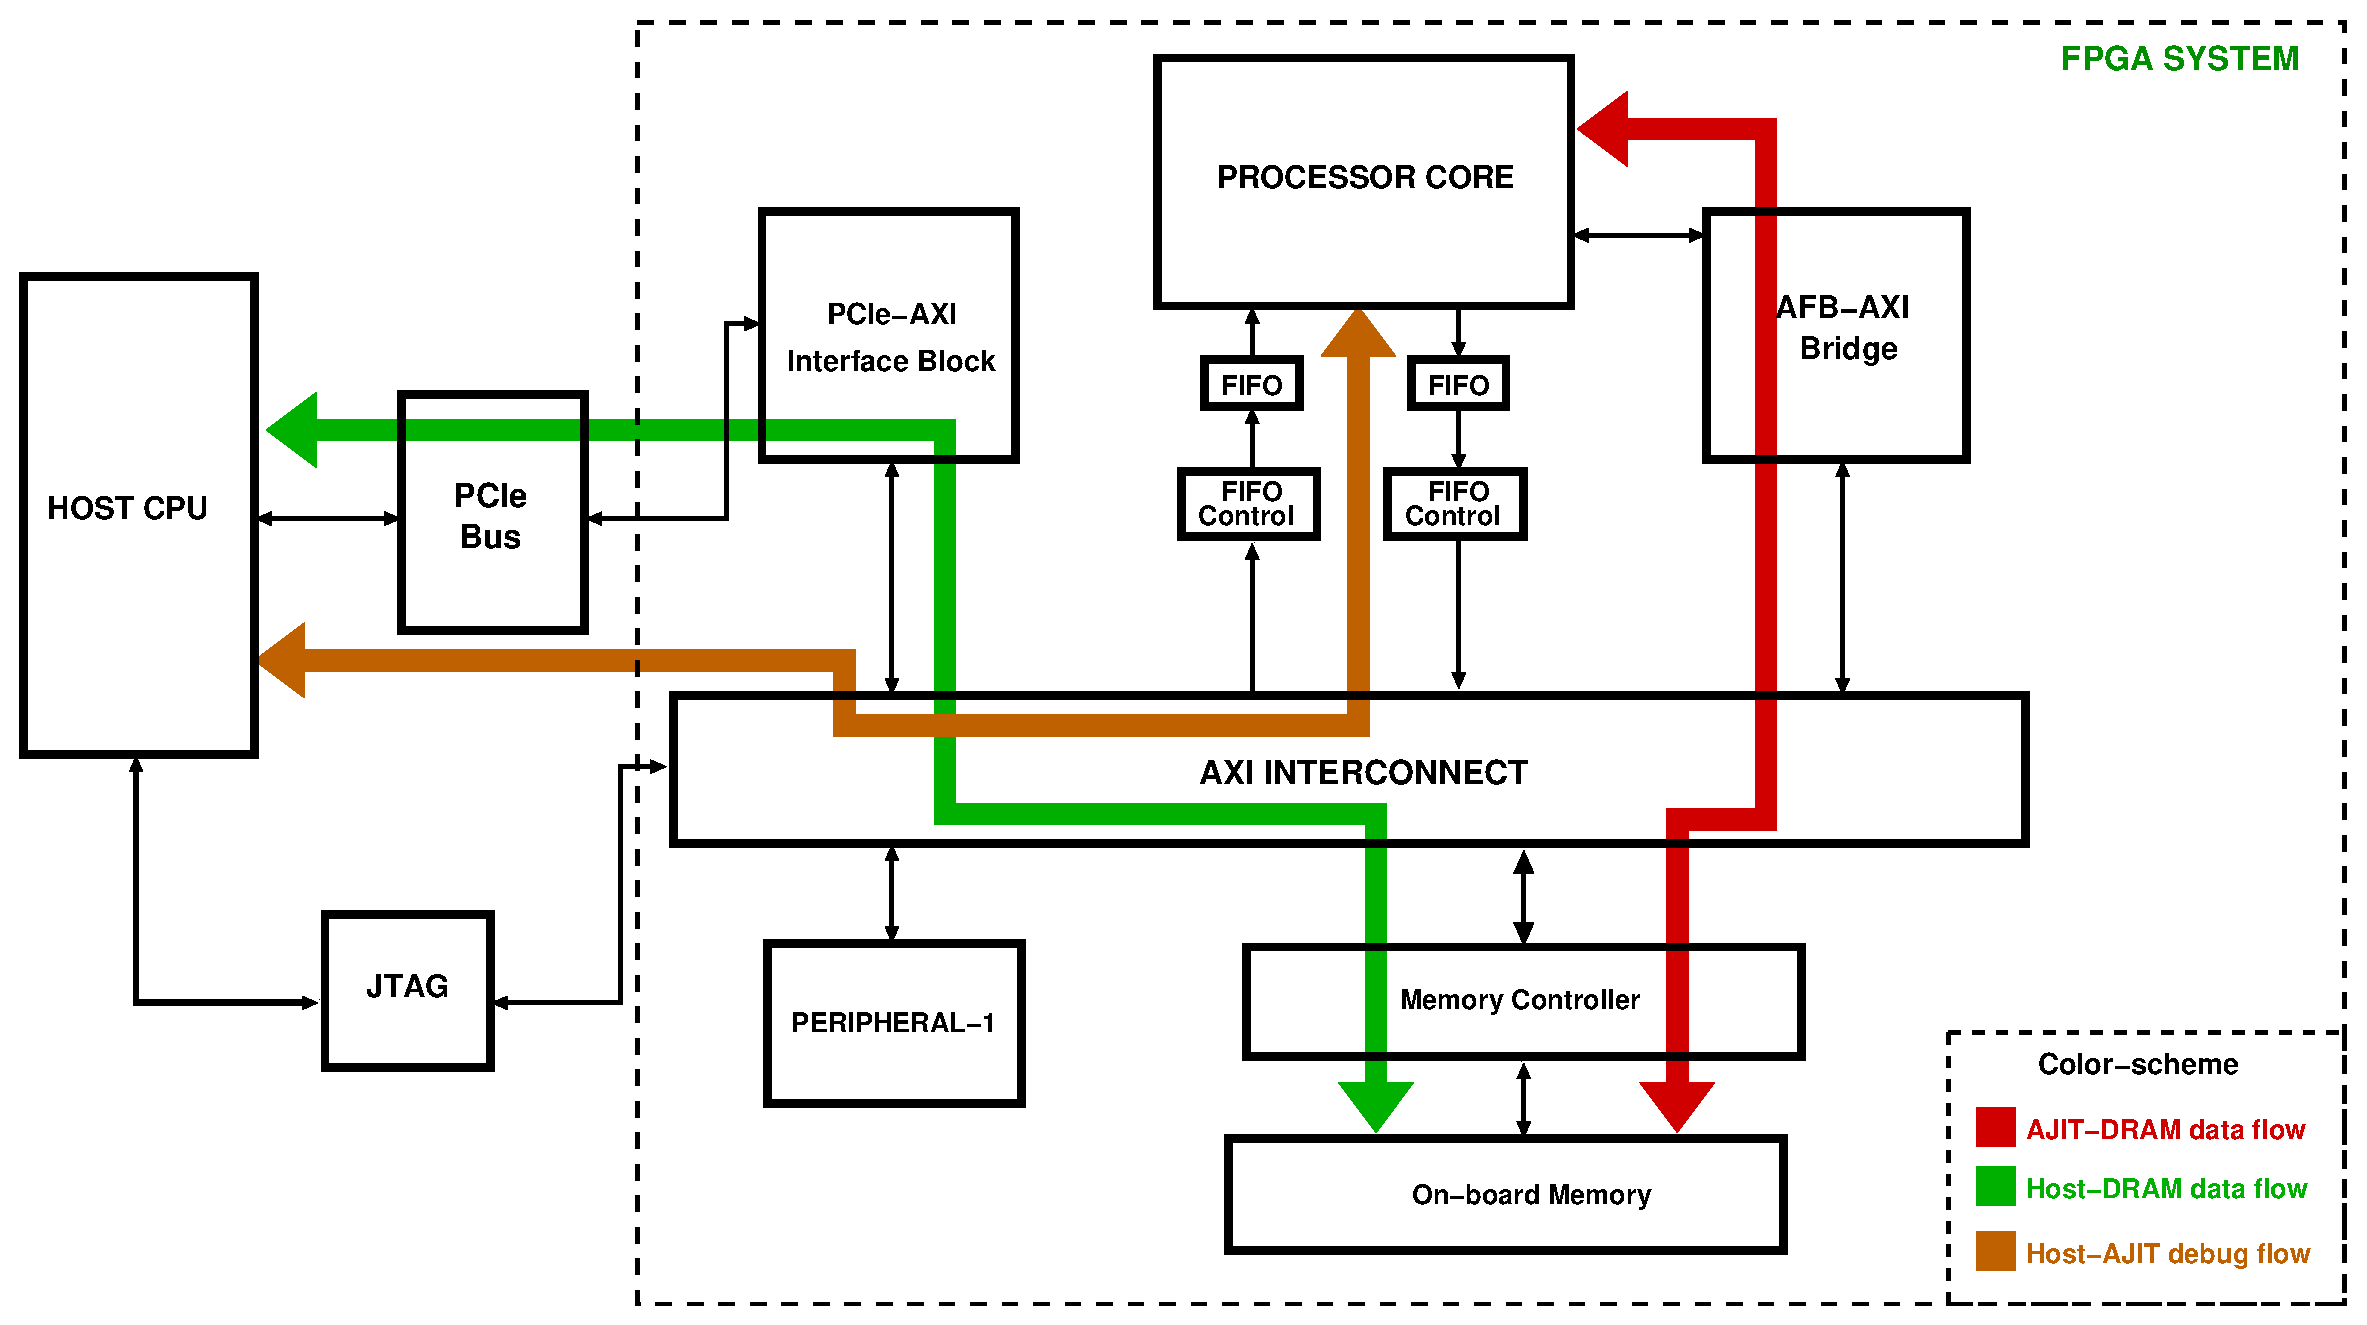
\includegraphics[width=\textwidth]{eps_pdf_sources/ajit_fpga/Full_System/Full_system_with_flow}
\caption{Complete FPGA system with data flow}
\label{full system with flow}
\end{figure}

\subsection{Testing of Interface}

We tested the interface using the XSCT command line utility which employs the JTAG interface and gives a direct access to all AXI
peripherals, an example of the same is shown in listing~\ref{lst:xsct}. 

\singlespacing
\scriptsize{
\begin{lstlisting}[language=bash, caption=xsct in action, label={lst:xsct}, emph={xsct, mrd, mwr}]
$ ä\textbf{xsct}ä
xsct% connect                                                                                                                                                             
attempting to launch hw_server
                                                                                                                                                                          
****** Xilinx hw_server v2017.1
  **** Build date : Apr 14 2017-19:01:52
    ** Copyright 1986-2017 Xilinx, Inc. All Rights Reserved.

INFO: hw_server application started
INFO: Use Ctrl-C to exit hw_server application

INFO: To connect to this hw_server instance use url: TCP:127.0.0.1:3121

tcfchan#0
xsct% target 3
xsct% mwr 0x80000000 0x01 
xsct% mrd 0x80000000
      0x01
\end{lstlisting}
}

\normalsize
\doublespacing

We also tested this with a PCI express interface from the Host CPU using the pcimem utility, an example of the same is shown in
listing~\ref{lst:pcimem}.

\singlespacing
\scriptsize{
\begin{lstlisting}[language=bash, caption=pcimem in action, label={lst:pcimem}, emph={resource0}]
$ ä\textbf{sudo ./pcimem /sys/bus/pci/devices/0000\:0a\:00.0/resource0 0 w}ä
  /sys/bus/pci/devices/0000\:0a\:00.0/resource0 opened.
  Target offset is 0x0, page size is 4096
  mmap(0, 134217728, 0x3, 0x1, 3, 0x0)
  PCI Memory mapped to address 0x4801f000.
  Value at offset 0x0 (0x4801f000): 0xC0BE0100
\end{lstlisting}
}
\normalsize
\doublespacing


%\chapter{Setup Specifications}

\section{Xilinx VC709}

\begin{table}[H]
\centering
\begin{tabular}{c | c}
\hline
Parameter & Spec-Description\\
\hline
FPGA Slices & xxxxx \\
DRAM Ports & 2 (4GB each) \\
On-board Clocks & xxxxx \\
PCIe compatible & xxxxx
\end{tabular}
\caption{VC709 Specifications}
\end{table}

\section{Host Machine}

\begin{table}[H]
\centering
\begin{tabular}{c | c | p{0.5\textwidth}}
\hline
Device & Spec & Comment \\
\hline
RAM & Corcix and 16GB & Relevant in order to run multiple Vivado instances\\
Motherboard & Intel Xeon some compatible shit & Limit of 128MB on BAR size\\ 
\end{tabular}
\caption{Host Machine Specifications}
\end{table}


\chapter{Software Interface}

\section{Driver Interface}
\subsection{Introduction}
The debug interface to the processor is a crucial part in development of applications as well as the development of the processor itself.
Here we attempt to provide a seamless debug interface which is easily extendible and integrable to the FPGA system and new processor cores.
The way the host machine communicates with the processor is by periodically sending and receiving packets of length 64-bits over the PCIe
bus of the host machine to the AXI interconnect on the FPGA system. The following figure shows the debug interface of the processor:-

\begin{figure}[H]
\centering
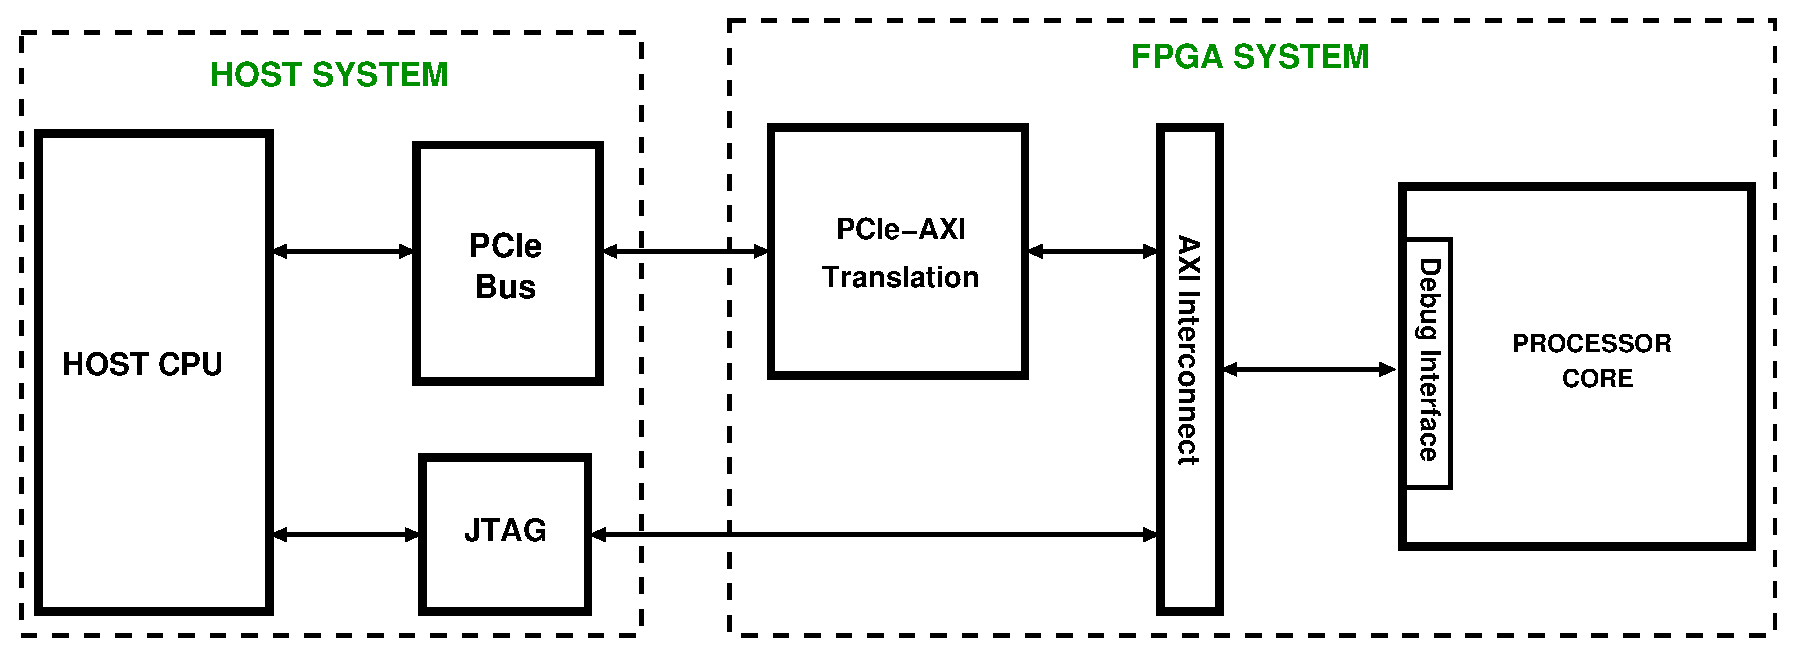
\includegraphics[width=\textwidth]{eps_pdf_sources/ajit_fpga/Debug_Interface/debug_channel_intro}
\caption{Debug channel from host to AJIT}
\end{figure}

\subsection{Testbench for the Driver Interface}
In order to test the FPGA system we run a software testbench on the host machine which controls the processor's mode and reads and writes
the on board memory. The driver API provides lower level function calls to the testbench in order to execute fundamental tasks on the FPGA system.
The testbench builds on this driver and contains a multi-threaded environment with several threads controlling their respective software
pipes which are then collected by the main thread to produce a 64-bit packet which contains the relevant Debug instruction for the processor
to execute. The driver API also aids development of userspace applications which need access to lower level FPGA system routines.

\begin{figure}[H]
\centering
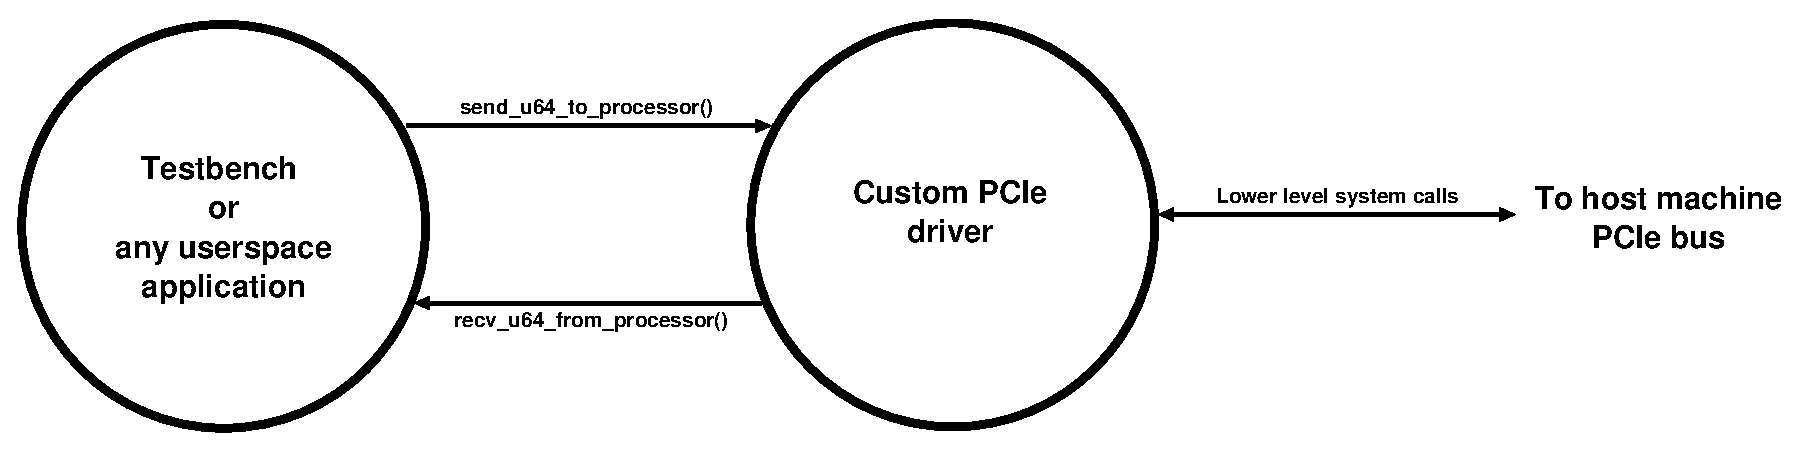
\includegraphics[width=\textwidth]{eps_pdf_sources/ajit_fpga/Software_Interface/testbench_and_application_illustration}
\caption{Driver API in action}
\end{figure}

\begin{figure}[H]
\centering
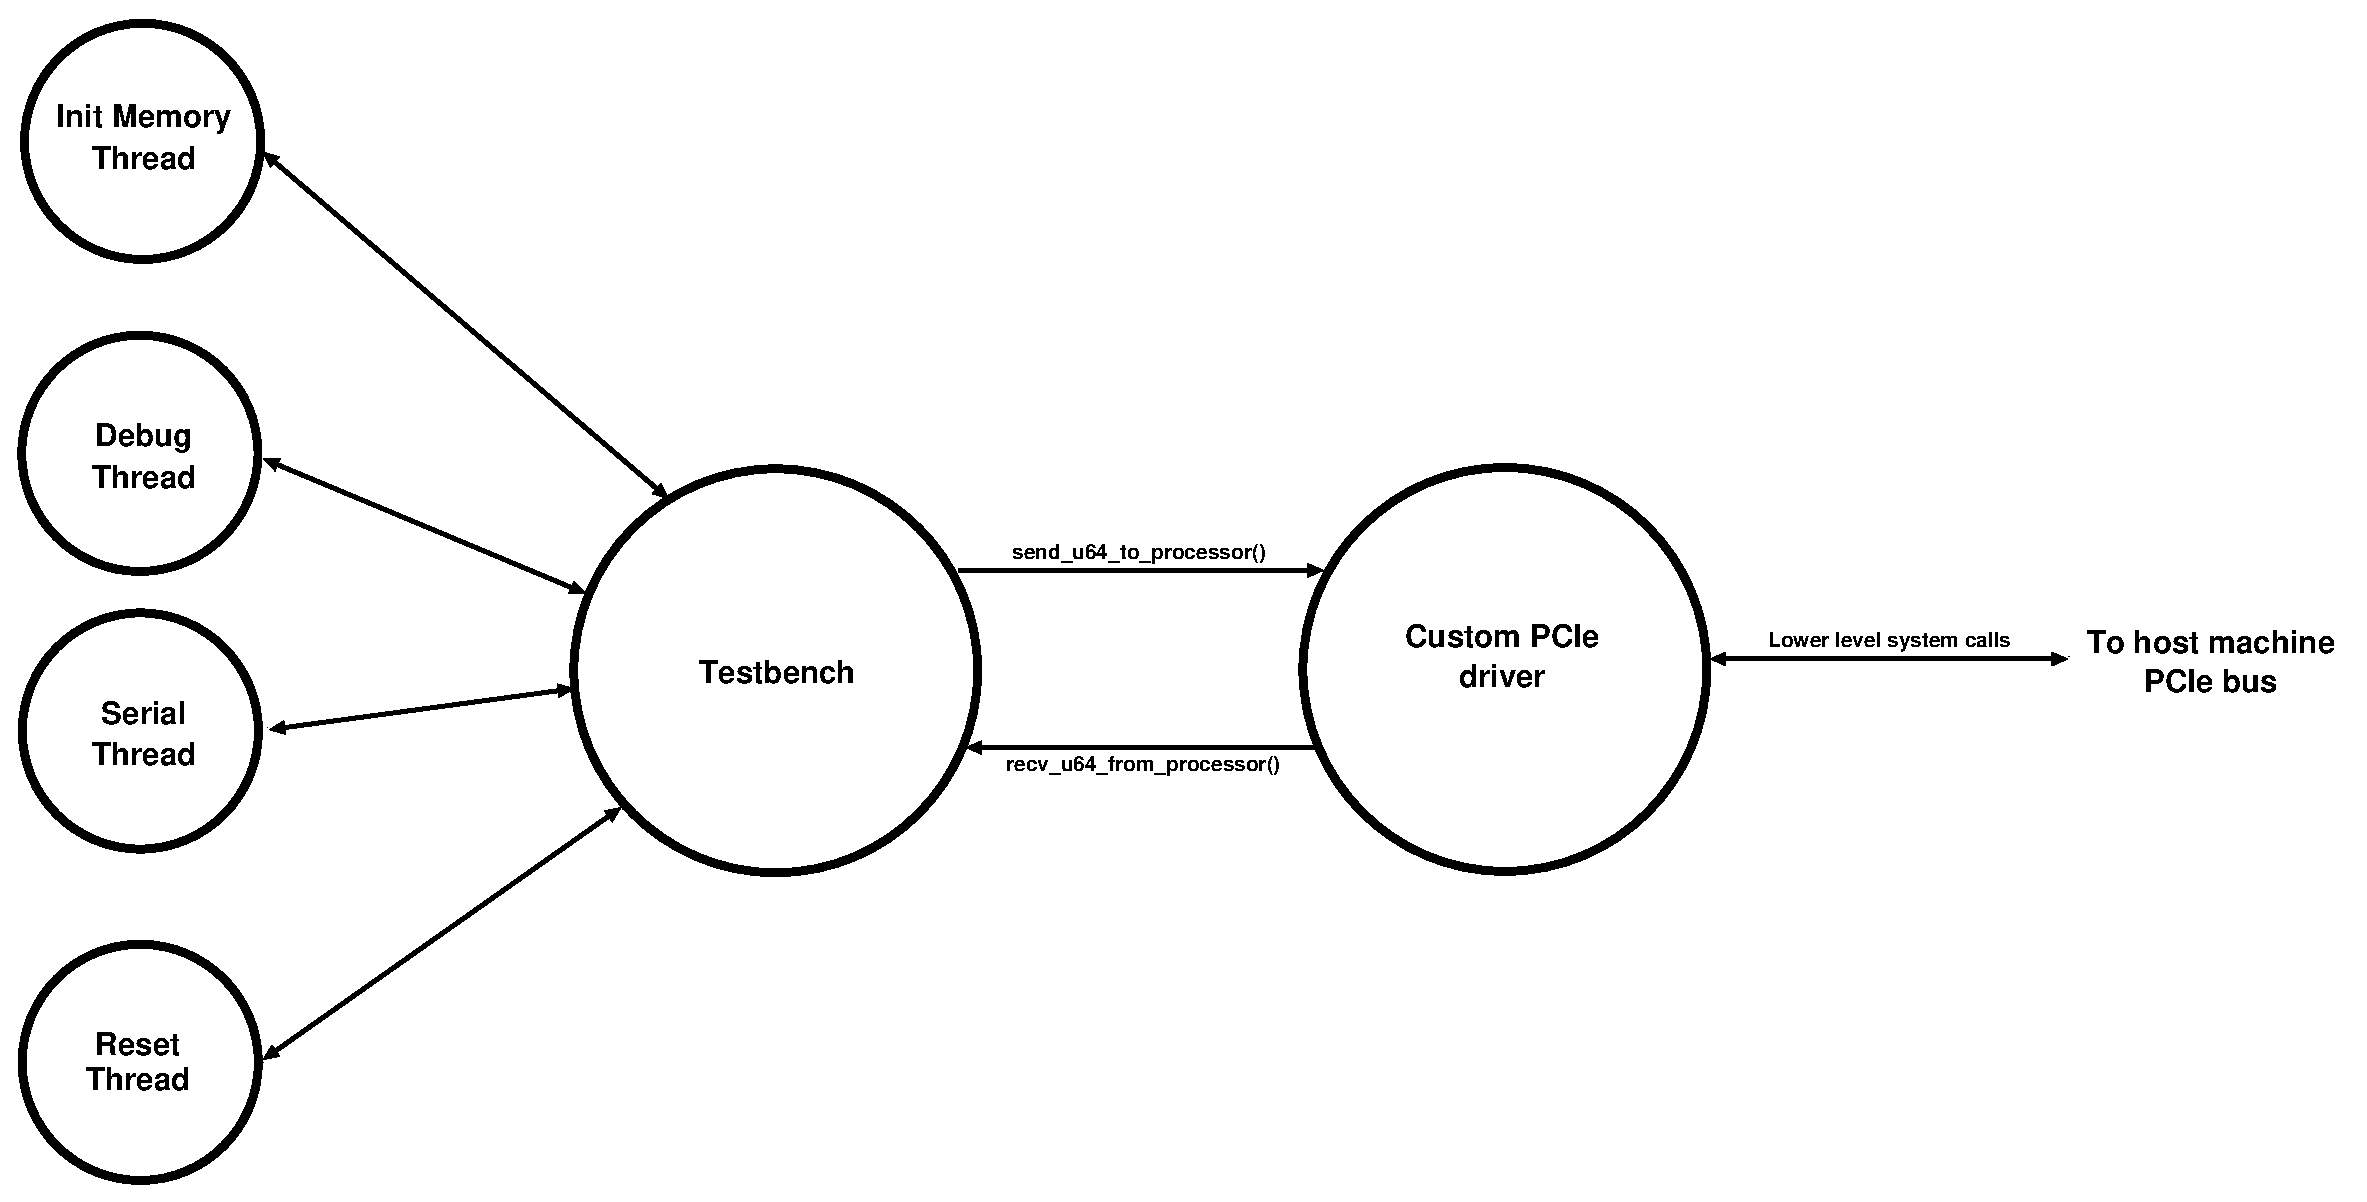
\includegraphics[width=\textwidth]{eps_pdf_sources/ajit_fpga/Software_Interface/testbench_illustration}
\caption{Software Testbench threads}
\end{figure}

%\begin{figure}[H]
%\centering
%\includegraphics[width=\textwidth]{eps_pdf_sources/ajit_fpga/Debug_Interface/aggregator_view}
%\caption{Driver API in action}
%\end{figure}

\section{Driver Interface discussion}

For the previous iteration of already developed software programs for AJIT to be compatible with the new FPGA model we need to keep the
identical call names to the API calls and need to have a Driver API interface which provides the same functions but with non-trivial and
different inherent implementations which is the multiple bars of 128MB one.

\section{Driver API}

The four black boxed functions that the API provides are:

\singlespacing
\scriptsize
\begin{lstlisting}[language=C, caption=Driver API]
void* initialize_axi_link(char* name){
...
}

int close_axi_link(void* fpga_device){
...
}

int write_to_axi_dram(void* fpga_device, uint32_t address, uint32_t write_word){
...
}

int read_from_axi_dram(void* fpga_device, uint32_t address, uint32_t *read_word){
...
}

int recv_u64_from_processor(uint64_t* r_word){
...
}

int send_u64_to_processor(uint64_t* s_word){
...
}
\end{lstlisting}
\normalsize
\doublespacing

\section{Driver development discussion}

Driver infrastructure can be broken down in four simple parts:\\

\verb|initialize_axi_link(...)| \\

As would be evident by the name this function, it initialize the axi link to a fpga device and returns the status of the opened device and prints error message if it
fails to open the device. It initializes an internal data structure specifically created to manipulate fpga devices, allocates memory and
returns a pointer to the created FPGA device.\\

\verb|close_axi_link(...)| \\

As would be evident by the name this function closes an already open fpga device and returns the status of the device and prints error
message if it fails to close the device. It frees the allocated memory for the internal data structure specifically created to manipulate
fpga devices, it returns a \verb|0| on successful freeing and hence closing of the connection FPGA.\\

\verb|write_to_axi_dram(...)|\\

This function provides the user with the functionality to write 32-bit words directly to the on-board DRAM by specifying the actual physical
DRAM address and the respective 32-bit word to be written. This will automatically find out the appropriate bar to be mapped to the host
memory and would write the word to the mmapped file and returns \verb|0| on a successful write.\\

\verb|read_from_axi_dram(...)|\\

This function provides the user with the functionality to read 32-bit words directly from the on-board DRAM by specifying the actual
physical DRAM address and the respective 32-bit word pointer to be stored with the read value. This will automatically find out the
appropriate bar to be mapped to the host memory and would read the word from the mmapped file and returns \verb|0| on a successful read.\\

\verb|send_u64_to_processor(...)| \\

This function is used to send a 64-bit word to the processor core. The approach here is to memory map the base address of the FIFO
controllers and providing the required offset to the data registers. For memory mapping we use \verb|mmap| with \verb|PROT_READ| and
\verb|PROT_WRITE| flags set so that we have the read-write access. We in effect get a pointer to the memory location of the data registers
which we can dereference to write our data which has been split into nibbles. This function after writing the data registers, polls the success bit in the
control register and as soon as it is set, the function returns the success status i.e. a \verb|0|. \\

 \verb|recv_u64_from_processor(...)| \\

This function is used to receive a 64-bit word from the processor core. The approach again here is to memory map the base address of the
FIFO controllers and providing the required offset to the data registers. For memory mapping we use \verb|mmap| with \verb|PROT_READ| and
\verb|PROT_WRITE| flags set so that we have the read-write access. This function before reading the data registers, polls the valid bit in
the control register and as soon as it is set the function reads the data in two chunks by reading the higher nibble and lower nibble
separately and then combines them to form the read 64-bit value.\\

\section{Explaining polling method}

The way in we perform a transfer of a 64-bit number is that we split it into two 32-bit numbers and write it out to 32 -bit memory mapped
registers inside the FIFO controllers from where the data is sent to the Debug FIFOs. For simplicity the driver currently continuously polls
the control register of the FIFO controllers and checks for the status bit to set and finishes the API call as soon it sets and returns the
received data/status dependent upon the API call made. 

\section{Need for interrupt based support in future}

To avoid the redundant polling approach we are going to introduce an interrupt based driver API which would would contain ISR routines
responding to the PCIe-AXI interface generated interrupts. For this functionality we most probably would need to have a Kernel Space
Module which would have direct access to Kernel ISR routines and would allow us to respond to specifically VC709 generated interrupts on
the PCIe bus in an efficient manner but this can in principle also be executed through user domain applications by registering the IRQ base
address as the interrupt base and writing an interrupt handler function and register it as the handler to this particular interrupt 

\section{Testing of the driver}

Preliminary tests were conducted using pcimem utility with successful results and extensive tests on the driver have been conducted using a
multithreaded software testbench which periodically sends and receives 64-bit packets from AJIT core.

\begin{displayquote}
A strong reference for this driver was a github project by the developer \verb|billfarrow| where he has provided the basis to read \& and write to
pci devices from a userspace domain.
\end{displayquote}


\chapter{Performance of the System}

%\section{Timing and utilization summary}

\section*{Timing Summary}

In the following table we report the timing summary of the synthesized and implemented design of the FPGA System on VC709 operating at
100MHz.

\begin{table}[H]
\centering
\begin{tabular}{c | c | c | c}
\hline
Parameter & Description & Tolerance & Value Obtained \\
\hline
WNS & Worst Negative Slack & 1-2 percent of 10ns & -0.1ns\\
CP & Critical Path & N/A & Exists within Xilinx Smartconnect  
\end{tabular}
\caption{Timing Summary}
\end{table}

\section*{Utilization Summary}
In the following table we report the utilization summary of the synthesized and implemented design of different variants of the FPGA System
on VC709.

\begin{table}[H]
\centering
\begin{tabular}{c | c | c}
\hline
Design & Description & Value Obtained \\
\hline
\end{tabular}
\caption{Utilization Summary}
\end{table}

\section*{Host to FPGA system}

\paragraph{Writing speed of PCIe\\}
\setlength{\parindent}{0em}
Writing speed of PCIe with 6 blocks of 128MB each after preliminary tests was found to be around 400 MB/s which is significantly higher than
the required speed in the current situation and also when compared to the past FPGA system. This speed is really helpful when we need to
write huge amount of data to memory for example to write the image of the custom compiled operating system for AJIT.

\paragraph{Reading speed of PCIe\\}

Reading speed of PCIe with 6 blocks of 128MB each after preliminary tests was found to be around 10 MB/s which is significantly higher than
the required speed in the current situation and also when compared to the past FPGA system. 


\chapter{Tests conducted}

\section{Indirect filling of on-board DRAM}

To check access of the host to the full 4GB on board DRAM Memory through a Memory Address Translator Block which Translates a read/write
request in form of two AXI slave register writes to an AXI Master request on the onboard AXI interconnect. It employs 3 registers to
accommodate address, data and type of request respectively. Figure~\ref{MAT flow} shows the flow for this indirect access to the on-board
DRAM through the Memory Address Translation block. More details have been provided in section~\ref{MAT block} regarding this block.

\begin{figure}[H]
\centering
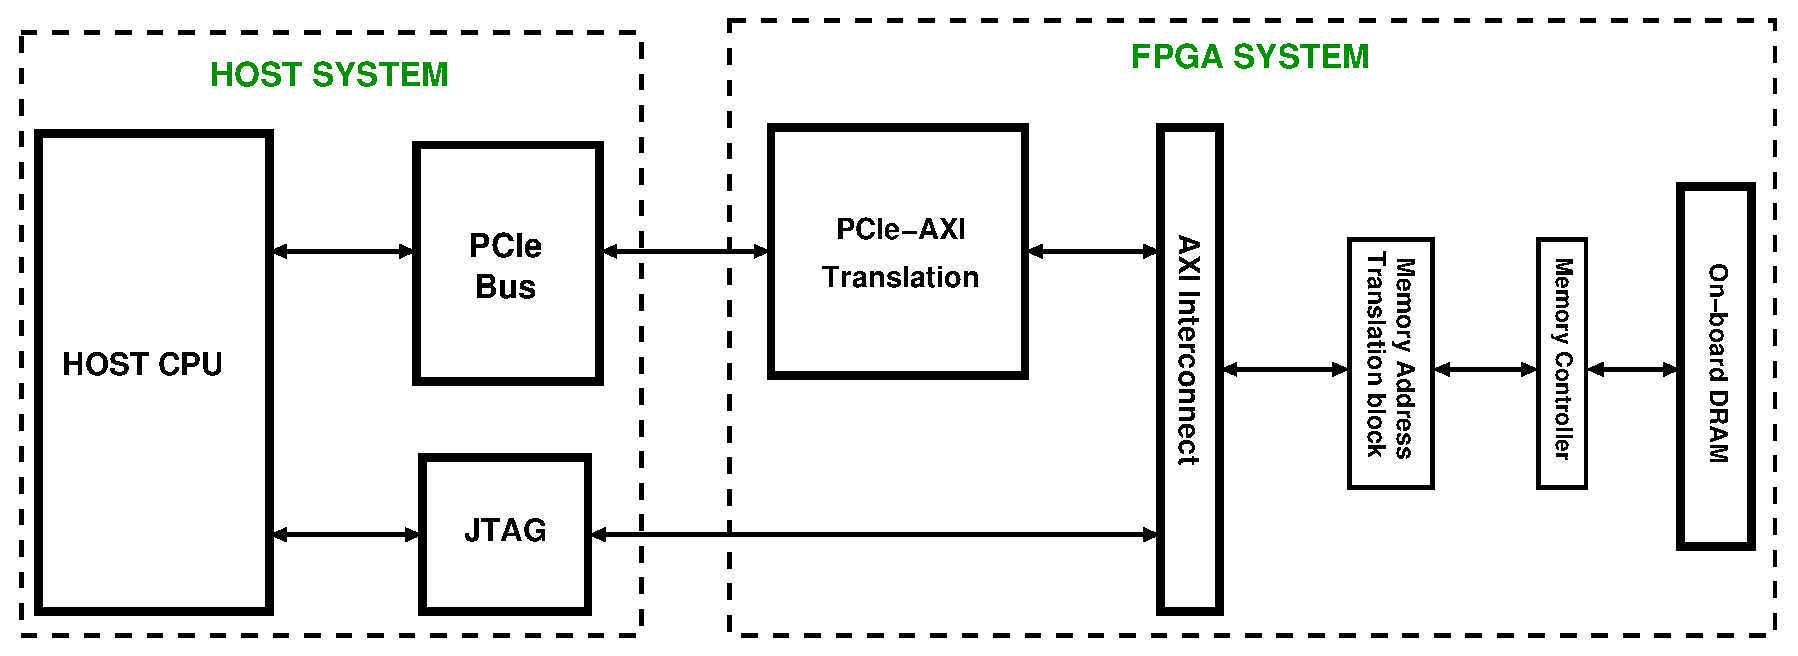
\includegraphics[width=\textwidth]{eps_pdf_sources/ajit_fpga/Tests_conducted/MAT}
\caption{Indirect memory channel from host to AJIT}
\label{MAT flow}
\end{figure}

\subsection{Results}

In order to write the whole 4GB memory through this block took around 45 minutes since in order to perform a single write to the on board
DRAM through this peripheral we need to perform 3 writes to this block including write address, write data and the type of request as write
into the AXI Slave registers of this block.

\section{March test on memory}

\subsection{What is March Test?}

A march test consists of a finite sequence of march elements. A march element is A finite sequence of Read and/or Write operations applied
to every cell in memory in either increasing address order (cell 0 to cell n-1) or decreasing address order (cell n-1 to cell 0). All
operations of a march element are done before proceeding to the next address. The march tests are a preferred method for RAM testing-Linear
complexity, regularity, and symmetry.

\subsection{Fault Models}
\begin{table}[H]
\begin{tabular}{c | m{0.7\textwidth}}
\hline
Fault Models & Description \\
\hline
Stuck-At Fault & The logic value of a line is always \textbf{0 or 1}\\
Transition Fault & A cell or a line that fails to undergo a $0 \rightarrow 1$ or a $1 \rightarrow 0$ transition \\
Coupling Fault & A write operation to one cell changes the content of a second cell other cells in the memory \\
NPS Fault & The content of a cell, or the ability to change its content, is influenced by the contents of some\\
Address Decodes Fault & With a certain address no cell will be accessed, a certain cell is never accessed, with a certain address multiple
cells are accessed simultaneously, and a certain cell can be accessed by multiple addresses
\end{tabular}
\caption{Fault Models}
\end{table}

\textit{NPS}: Neighbourhood Pattern Sensitive

\subsection{Our Implementation}
Here we perform the standard March test on the on board DRAM memory by accessing it from the host using the 6 PCIe BARS created as PCIe
resources on the /sys path of Linux. Here is a screenshot showing the resource files. We implement the \textbf{March X} algorithm because it
is an $O(n)$ time algorithm and covers most of the basic faults.

\begin{algorithm}
\caption{March X algorithm}\label{March X}
\begin{algorithmic}[1]
\State Step 1: \textbf{write} 0 with up addressing order;
\State Step 2: \textbf{read} 0 and \textbf{write} 1 with up addressing order;
\State Step 3: \textbf{read} 1 and \textbf{write} 0 with down addressing order;
\State Step 4: \textbf{read} 0 with down addressing order;
\end{algorithmic}
\end{algorithm}

\subsection{Faults covered}
The above algorithm covers Address Decoder Faults, Stuck at Faults, Transition Faults and some coupling faults.

\subsection{Timing Results}

The below table consists of the time taken by the host to conduct the March test on each bar of the on-board memory.

\begin{table}[H]
\centering
\begin{tabular}{c | c}
\hline
BAR ID & Time Taken(in sec) \\
\hline
BAR0 & 59.658342534 \\
BAR1 & 59.640203597 \\
BAR2 & 59.607970220 \\
BAR3 & 59.611384216 \\
BAR4 & 59.690874289 \\
BAR5 & 59.722889924
\end{tabular}
\caption{Timing Results}
\end{table}


\chapter{Alternate Designs}

\section{Single bar of 4GB}

The first approach in an attempt to interface the full range of on-board DRAM i.e. 4GB to the host machine was made in a straight forward
fashion by keeping a single bar of size 4GB the PCIe interface and it was expected that then by memory mapping by the thus generated
\verb|/sys/resourceX| files(where \verb|X| is an integer) generated by the PCIe-AXI IP would give the whole access to whole DRAM. But even
on repeated attempts of sucessful hardware desgins we could not make the PCIe interface to generate a resource file of size 4GB. At first
this was suspected as an operating system issue but after further digging we found that the usual devices on PCIe bus of this machine had
memory regions of the scale 16MB, 32MB going as far as 64MB. Hence we brought down our bar sizes to 128MB after some trial and error we
found by experimentation that the motherboard had a limit on the BAR sizes of 128MB.We tried multiple BARS of smaller size i.e. 4K, 32MB etc
until we arrived at 128MB limit. This happened out of necessity and lack of open documentation over the internet for the host motherboard.

\pagebreak

\section{Memory Address Translator block} \label{MAT block}

To check access of the host to the full 4GB on board DRAM Memory through a Memory Address Translator Block which Translates a read/write
request in form of two AXI slave register writes to an AXI Master request on the onboard AXI interconnect. It employs 3 registers to
accommodate address, data and type of request respectively. The listing~\ref{lst:MAT} provides the HLS design code for this block and
employs similar pragma statements as explained before.

\singlespacing
\scriptsize
\begin{lstlisting}[language=C++, caption=Memory Address Translator HLS, label={lst:MAT}]
#include "ap_int.h"
#include "hls_stream.h"

void Memory_Address_Translator(int data_in,int address,int* translated_base,...,int *data_out)
{
	#pragma HLS INTERFACE m_axi port=translated_base offset=none
	#pragma HLS INTERFACE s_axilite port=data_in
	#pragma HLS INTERFACE s_axilite port=address
	#pragma HLS INTERFACE s_axilite port=read_write_in
	#pragma HLS INTERFACE s_axilite port=data_out
	#pragma HLS INTERFACE s_axilite port=return
	
	// read_write_in is 1 for write and 0 for read

	if(read_write_in)
	{
		translated_base[address/4] = data_in;
	}
	else
	{
		*data_out = translated_base[address/4];
	}
}
\end{lstlisting}
% void Memory_Address_Translator(int data_in, int address, int* translated_base,int read_write_in, int *data_out)
\normalsize
\doublespacing


\section{Memory Copier Block}

This block serves as a small DMA, it will copy a block of 128MB of data from one address in memory into another. The 32-bit source and
destination addresses and the read/write type request can be written into AXI Slave registers through the host machine over PCIe interface.
It translates the required addresses and the type of request to an AXI Master request on the interconnect. This block was created as an
alternative way to access the whole on-board DRAM from the host machine when the host motherboard was found to have a limit of 128MB on the
size of \verb|/sys/resourceX| files(where \verb|X| is an integer) generated by the PCIe-AXI IP. The listing~\ref{lst:MCB} provides the HLS
design code for this block and employs similar pragma statements as explained before.

%- Need a diagram to explain the flow of this block
\singlespacing
\begin{lstlisting}[language=C++, caption= Memory Copier Block HLS, label={lst:MCB}]
#include <ap_int.h>
#include <hls_stream.h>
#include <string.h>

void hls_dma (char *pSrc, char *pDest) {
    #pragma HLS INTERFACE s_axilite port=return
    #pragma HLS INTERFACE m_axi port=pSrc offset=slave
    #pragma HLS INTERFACE m_axi port=pDest offset=slave
    for (int i = 0; i < 1024*1024*128; i++) {
        pDest[i] = pSrc[i];
    }
}
\end{lstlisting}
\doublespacing



\chapter{Current and expected problems}

\section{Expected Problems}

\subsection{Read speed over PCIe}

The current data reading speed offered over PCIe by the test setup is around 10MB/s which is more than enough required by the debugging
interface of AJIT processor which is around 40 KB/s. But this is considerably less when compared to the write speed offered over the same
bus which is around 400 MB/s. This could be a bottleneck in the future if we higher speeds are required over the debug interface of AJIT
processor.

\section{Addressed Problems}

\subsection{Motherboard memory space limit for PCIe bars}

The first approach in an attempt to interface the full range of on-board DRAM i.e. 4GB to the host machine was made in a straight forward
fashion by keeping a single bar of size 4GB the PCIe interface and it was expected that then by memory mapping by the thus generated
\verb|/sys/resourceX| files(where \verb|X| is an integer) generated by the PCIe-AXI IP would give the whole access to whole DRAM. But even
on repeated attempts of successful hardware designs we could not make the PCIe interface to generate a resource file of size 4GB. At first
this was suspected as an operating system issue but after further digging we found that the usual devices on PCIe bus of this machine had
memory regions of the scale 16MB, 32MB going as far as 64MB. Hence we brought down our bar sizes to 128MB after some trial and error we
found by experimentation that the motherboard had a limit on the BAR sizes of 128MB.We tried multiple BARS of smaller size i.e. 4K, 32MB etc
until we arrived at 128MB limit. This happened out of necessity and lack of open documentation over the internet. For example on two
different systems in EE department in IIT Bombay we found first machine's motherboard has a limit of 128MB bar size whereas another machine
has a limit of 256MB bar size. This makes the whole FPGA design scalable in terms of memory size and we can have the access to the whole 4GB
memory on a recent versioned motherboard.

\subsubsection{Vivado putting random errors and resolving it by redundant actions}
Updation command offered by Vivado when run on project sources messes up sometimes to update the rebuilt custom IPs and shows that those IPs
have been locked and sometimes not found. This is mostly solved by checking permissions for the IP files or by repackaging the custom IPs or
by reloading the whole project.


\part{Convolution Engine}

\chapter{Introduction}

\section{Introduction to AJIT}

AJIT is an indigenous processor which has been designed at IIT Bombay and is currently in its second design and manufacturing iteration.
AJIT is based on the open SPARC-v8 ISA and is currently a 32-bit processor. The current design runs at 100 MHz and has been manufactured at
SCL, Chandigarh using the 180nm technological node.

\begin{figure}[H]
\centering
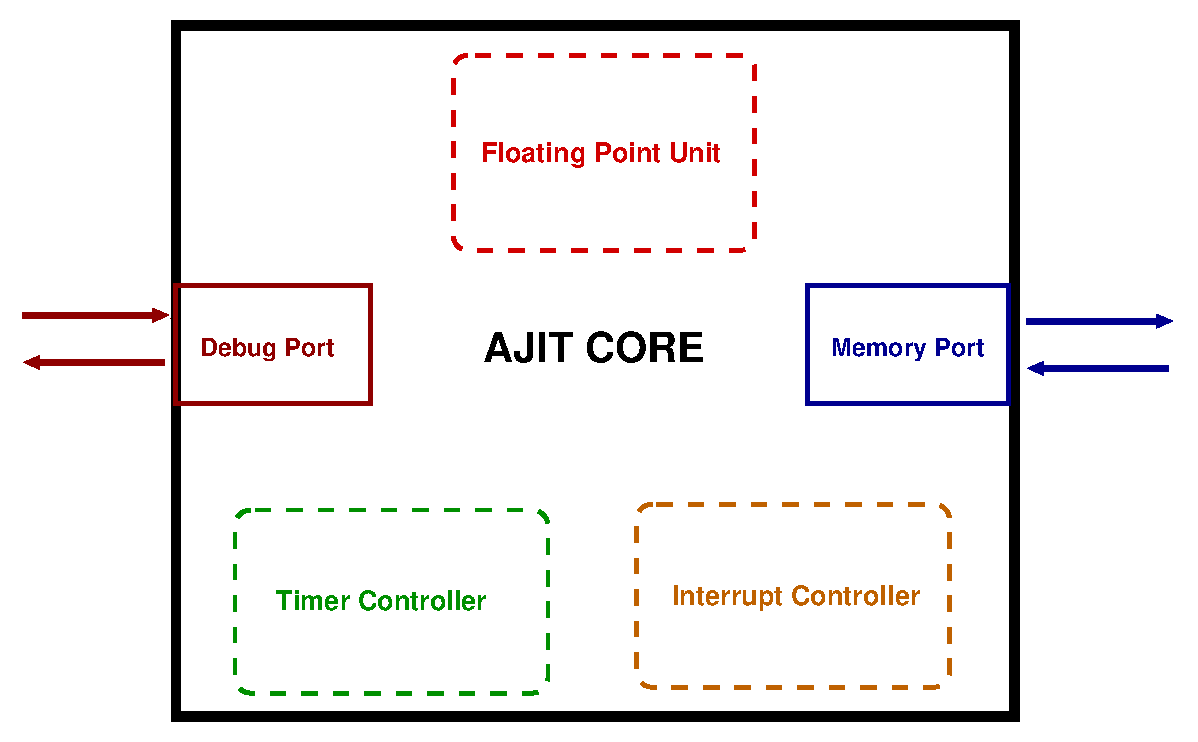
\includegraphics[scale=0.7]{eps_pdf_sources/ajit_fpga/AJIT/ajit_intro}
\caption{Overview of AJIT}
\end{figure}

\subsection{Support for AJIT}

AJIT has a functionally correct and verified C model which is used to verify new additions to the processor and user space
applications. AJIT also has a VHDL model which we incorporate into the later stages of this project and the same model later on loads
different programs ( before testing loading of an OS ) directly from the DRAM. 

\section{Introduction to the Project}

The main aim of this project is to provide an alternative to an earlier FPGA model designed around AJIT processor which had limited
on-board memory of 4MB and hence could borderline load a Linux system since the minimum memory requirement for a Linux operating system to
boot is around 4MB. The operating system thus loaded/booted had very limited kernel modules and userspace drivers to interface with hardware
elements.\\

This project is focussed at leveraging high DRAM storage capabilities and the high read and write speed of PCIe bus of the Xilinx VC709
board in order to make it capable to boot a heavily loaded embedded OS( quite possibly an RTOS ) with all the basic kernel modules and
userspace drivers to interface with hardware elements such as networking.\\

This process of booting an embedded OS on a FPGA platform is really advantageous as compared to booting OS on development boards based
around ASICs as we outline later. This project aims to integrate this FPGA system with a \verb|C++| based application to implement
a router system down the line.\\

We aim to incorporate soft core peripherals such as a Ethernet controller, USB controller etc to this FPGA system to ease the access to the
system through \verb|ssh| connections or through \verb|serial| connections. These kinds of easily integrable peripherals are expected to
make the development of custom applications really swift.\\

This project as we demonstrate later can also be used as a test-bed for HPC codecs development and testing. These peripherals can be
distributed along with the AJIT processor as part of its HPC peripheral library.


%\chapter{Need for a HPC engine}


%\chapter{Specifications}

Following is the specification for the current storage of image and kernel data:-

\begin{itemize}

\item 8 bits per pixel of image data and also kernel data.
\item Image would be of size 1024 x 1024 pixels (Basically 1022x1022 with zero padding).
\item Kernel would be of size 3 x 3.

\end{itemize}

Following is the specification for the current convolution core:- 

\begin{itemize}

\item An AXI Slave interface as the input interface for the addresses for the fetcher.
\item 32 coprocessors each assigned 32 rows by the fetcher.
\item A FIFO like interface for the fetcher to interface with the convolution core.
\item An AXI Master port for the fetcher for performing write backs to the memory.

\end{itemize}


\chapter{Design of the Engine}

\section*{Specifications}

Following is the specification for the current storage of image and kernel data:-

\begin{itemize}

\item 8 bits per pixel of image data and also kernel data.
\item Image would be of size 1024 x 1024 pixels (Basically 1022x1022 with zero padding).
\item Kernel would be of size 3 x 3.

\end{itemize}

Following is the specification for the current convolution core:- 

\begin{itemize}

\item An AXI Slave interface as the input interface for the addresses for the fetcher.
\item The number of coprocessors are kept variable to compare performance and hardware resource consumption.
\item A FIFO like interface for the fetcher to interface with the convolution core.
\item An AXI Master port for the fetcher for performing write backs to the memory.

\end{itemize}

\section{Storage design for image data}

The data is stored row wise as shown in the figure below. This strategy was opted to make the fetch and write back protocol really
straight-forward. The core gets the address of the first element of the first row of the image matrix, and of the kernel matrix and also the
physical address of the write back location in the DRAM.

\section{Fetch policy for the engine}

The fetch policy for the core is includes fetching the kernel data first and sending it out to all the coprocessors inside the core. After
this the fetching of image data begins and here we play a little smart and fetch 4 bytes of data in every memory read call and split the
data within the core to segregate the individual pixel data. 

\section{Number of coprocessors}

Since the image is chosen to be of size 1024x1024 it seems really convenient to have a number of coprocessors which is a factor of 1024. To
keep it symmetric we have kept the number of coprocessors to be 1, 2, 4, 8, 16 and 32 so that a single model of coprocessor can be
replicated in an convenient manner. Each coprocessor is fed with x rows of image data and the coprocessors are started in parallel, here x is
dependent on the number of operational coprocessors in the design.

\section{Flow design}

Figure~\ref{convolution core} represents the internal flow of the generic convolution engine which employs a variable number of cores since
we will utilize this to employ this design to test the performance and hardware consumption on a range of number of coprocessors. As can be
seen the core has a fetch unit which is responsible for fetching the incoming data from the input pipe to the core and distributing the work
between all the operational cores one by one and then collecting back the results from each of their output pipes and writing it back to the output pipe
of the core. Each coprocessor is designed to convolve the incoming image data with an initially stored kernel and write back the result to
its respective output pipe. The coprocessor model is discussed later on and we also dive down into the internal design of the coprocessor
when we discuss about improving its design efficiency and throughput.

\begin{figure}[H]
\centering
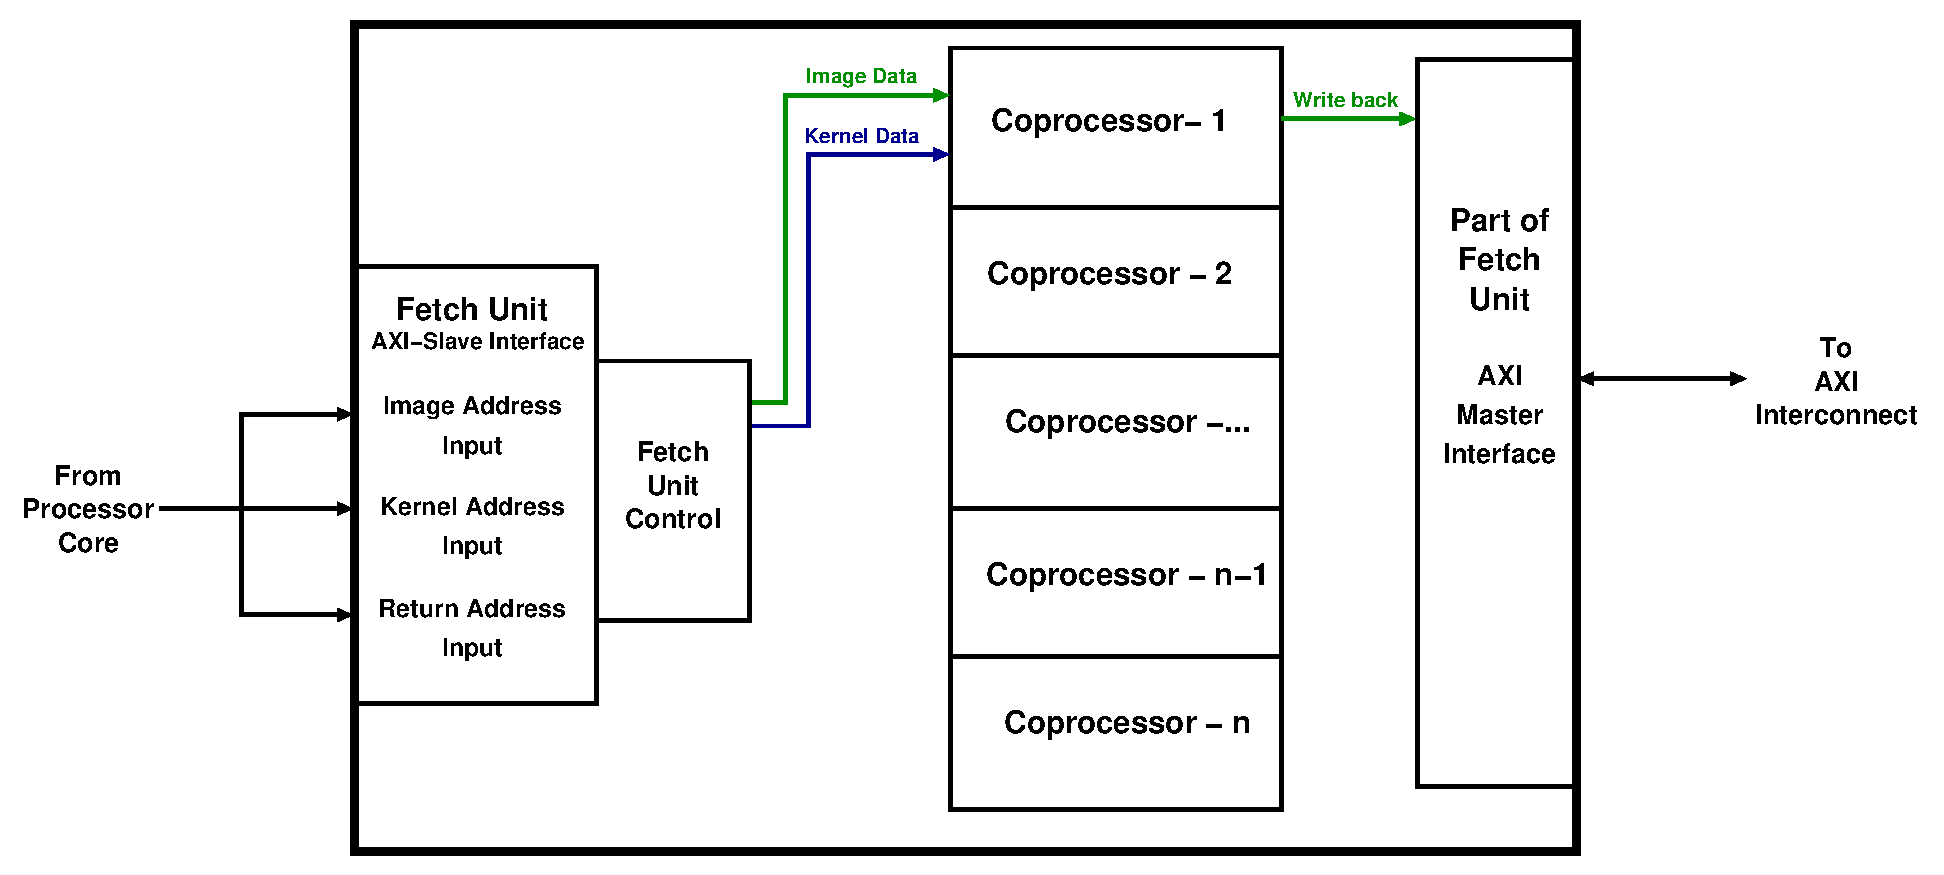
\includegraphics[scale=0.5]{eps_pdf_sources/convolution_engine/core}
\caption{Core Design}
\label{convolution core}
\end{figure}

\onehalfspacing
Figure~\ref{full system integrated with convolution engine} shows a sample system which could be built to integrate the convolution engine
with the AJIT FPGA system. The convolution engine can be controlled by AJIT and can also be directly tinkered with from the host machine
through the PCIe-AXI block. The engine can be assigned a task to perform a convolution from a software application by first storing the
relevant data in DRAM by \verb|write_to_axi_dram| call from the driver API and then the results can be read back using the
\verb|read_from_axi_dram| call.

\begin{figure}[H]
\centering
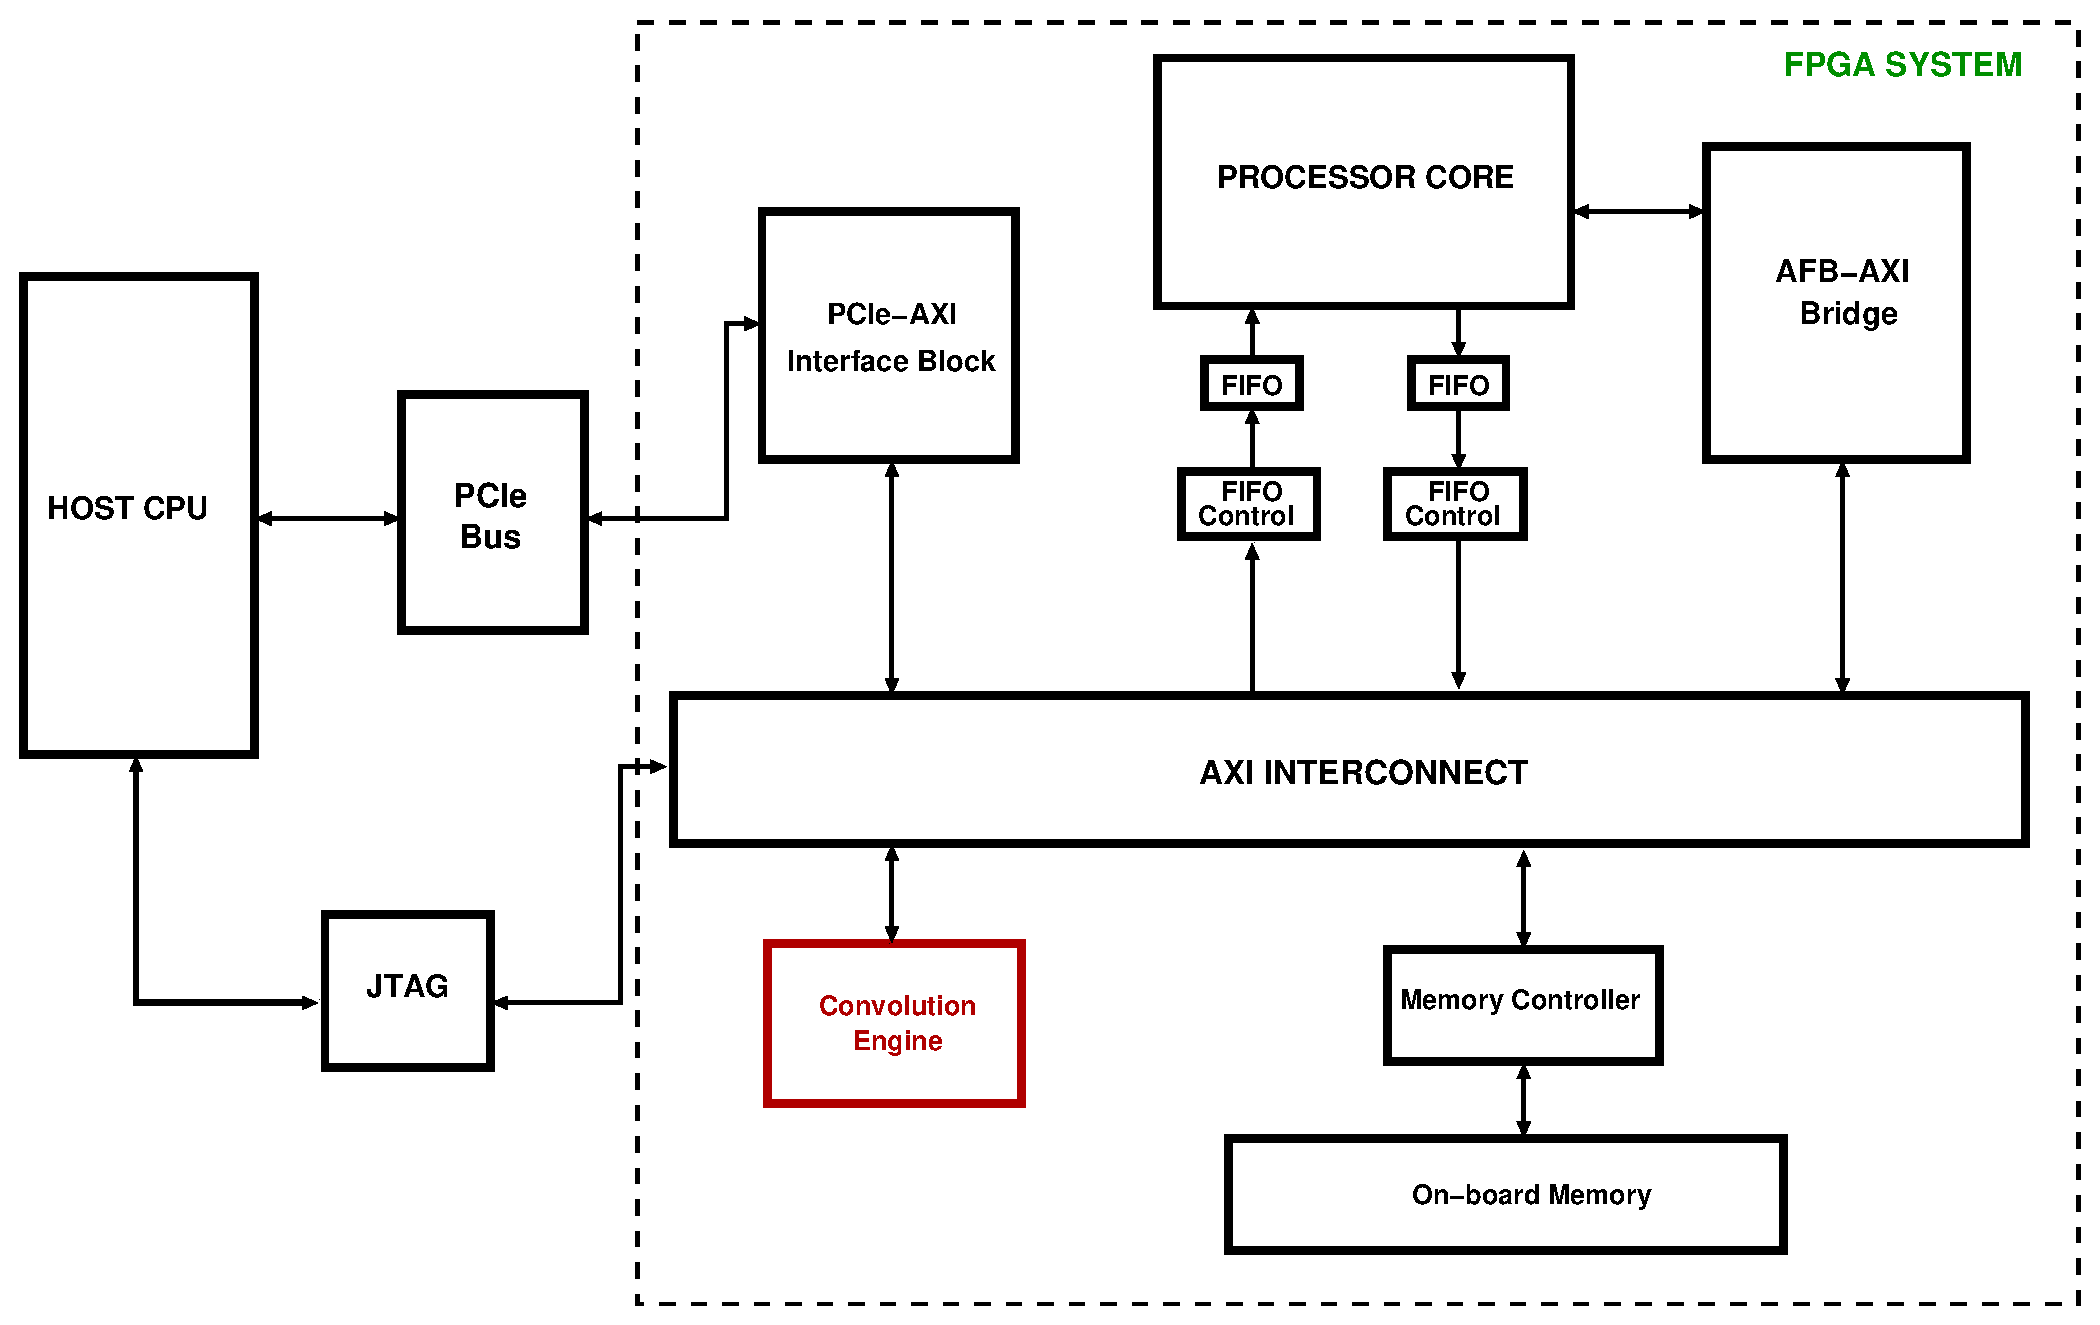
\includegraphics[width=\textwidth]{eps_pdf_sources/convolution_engine/Full_system_integrated_with_core}
\caption{Complete FPGA system with data flow}
\label{full system integrated with convolution engine}
\end{figure}

\doublespacing


\chapter{Implementation}

\section{Vivado HLS}

Listing~\ref{lst:convolution_engine_vivado_hls} shows the convolution engine design which would convolve a 1024$\times$1024 image with a
3$\times$3 kernel. This is a functionally correct but an unoptimized design for the convolution engine of this size.

\singlespacing
\scriptsize
\begin{lstlisting}[language=C++, caption=Core Vivado HLS, label={lst:convolution_engine_vivado_hls}]
#include "ap_int.h"
#include "hls_stream.h"

void core(char* init_row, char* kernel_data_row, char* row_dest) {
    #pragma HLS INTERFACE s_axilite port=return
    #pragma HLS INTERFACE m_axi port=init_row offset=slave
    #pragma HLS INTERFACE m_axi port=kernel_data_row offset=slave
    #pragma HLS INTERFACE m_axi port=row_dest offset=slave

    // assume an image size of 3x3 for now and the image is already padded with zeros.
    // assuming a kernel of size 3x3 which is symmetric or already flipped stored at 
    // the kernel storage location.

    // init_row points to a 5x5 image matrix in hardware.

    char i,j;
    char index=0;
    char acc=0;
    char rows = 3; 
    char cols = 3;

    for(i=0;i<rows;i+=rows)
    {
	for(j=0;j<cols;j++)
	{
		acc+= kernel_data_row[0]*(*(init_row+i+j));
		acc+= kernel_data_row[1]*(*(init_row+i+j+1));
		acc+= kernel_data_row[2]*(*(init_row+i+j+2));
		acc+= kernel_data_row[3]*(*(init_row+i+rows+j));
		acc+= kernel_data_row[4]*(*(init_row+i+rows+j+1));
		acc+= kernel_data_row[5]*(*(init_row+i+rows+j+2));
		acc+= kernel_data_row[6]*(*(init_row+i+2*rows+j));
		acc+= kernel_data_row[7]*(*(init_row+i+2*rows+j+1));
		acc+= kernel_data_row[8]*(*(init_row+i+2*rows+j+2));
		row_dest[index] = acc;
		index++;
	}
    }
}
\end{lstlisting}
\normalsize
\doublespacing


\section{AHIR HLS}

\subsection{C to VHDL}
\subsubsection{Non-pipelined Version}

\subsubsection{Pipelined Version}

\subsection{Aa to VHDL}
\subsubsection{Non-pipelined Version}

\subsubsection{Pipelined Version}

\section{Testing Setup}

\subsection{AHIR Testbenches}

\subsubsection{Hardware Test}

\paragraph{testbench\_hw \\}
\blindtext
\paragraph{ ahir\_system\_test\_bench \\}

\subsubsection{Software Test}

\paragraph{testbench\_sw \\}



\chapter{Hardware Usage comparison}

\section{Background}

Here we compare the hardware resources required by the HDL design generated by Vivado HLS and Aa HLS implementation of the same core.
Also within the Aa HLS implementation we compare the hardware resources required by the Pipelined version of the core with the Non-pipelined
version of the core by varying the number of coprocessors utilized in development of the internal architecture of the core. The default
pipeline depth is currently kept at 7 to produce the following values and plots.

%\section{Vivado HLS Implementation}
%\blindtext

\section{AHIR HLS Implementation}

Here we produce the results from the synthesis and implementation of different variants of our convolution engine where we consider the
number of Flip Flops in the implemented design as our metric to measure the hardware usage of each variant. We produce pipelined and
non-pipelined variants for a given number of coprocessors through two methods namely C HLS and Aa HLS(described in previous chapter).
Through this process we aim to show the advantage of generating a hardware system through Aa HLS instead of C HLS.The board chosen for this
process was Xilinx's VC709.

%\pagebreak

\subsection{C to VHDL}

\subsubsection*{Non-pipelined Version}

\begin{table}[H]
\centering
\begin{tabular}{c|c}%
    \hline
    \bfseries Number of Cores & \bfseries FFs\\\hline % specify table head
    \csvreader[head to column names]{csvs/c_np.csv}{}% use head of csv as column names
    {\\\cores & \ffs} % specify your coloumns here
\end{tabular}
\caption{Hardware Resources}
\end{table}

\plotfromcsv{csvs/c_np.csv}{Non-pipelined Coprocessor}

\subsubsection*{Pipelined Version}

\begin{table}[H]
\centering
\begin{tabular}{c|c}%
    \hline
    \bfseries Number of Cores & \bfseries FFs\\\hline % specify table head
    \csvreader[head to column names]{csvs/c_p.csv}{}% use head of csv as column names
    {\\\cores & \ffs} % specify your coloumns here
\end{tabular}
\caption{Hardware Resources}
\end{table}

\plotfromcsv{csvs/c_p.csv}{Pipelined Coprocessor}

\subsection{Aa to VHDL}

\subsubsection*{Non-pipelined Version}

\begin{table}[H]
\centering
\begin{tabular}{c|c}%
    \hline
    \bfseries Number of Cores & \bfseries FFs\\\hline % specify table head
    \csvreader[head to column names]{csvs/aa_np.csv}{}% use head of csv as column names
    {\\\cores & \ffs} % specify your coloumns here
\end{tabular}
\caption{Hardware Resources}
\end{table}

\plotfromcsv{csvs/aa_np.csv}{Non-pipelined Coprocessor}

\subsubsection*{Pipelined Version}

\begin{table}[H]
\centering
\begin{tabular}{c|c}%
    \hline
    \bfseries Number of Cores & \bfseries FFs\\\hline % specify table head
    \csvreader[head to column names]{csvs/aa_p.csv}{}% use head of csv as column names
    {\\\cores & \ffs} % specify your coloumns here
\end{tabular}
\caption{Hardware Resources}
\end{table}

\plotfromcsv{csvs/aa_p.csv}{Pipelined Coprocessor}


%\chapter{Testing Setup}

\section{AHIR Testbenches}

\subsection{Hardware Test}

- testbench\_hw \\
- ahir\_system\_test\_bench \\

\subsection{Software Test}

- testbench\_sw \\



%\chapter{Performance Comparison Between Software \& Hardware}


%\chapter{Results}

\section{Timing Results}

Timing results from different variants of the engine design for convoluting an image of size 1024$\times$1024 with a kernel of size
3$\times$3. 

\subsection{C to VHDL}

\subsubsection*{Non-pipelined Version}

\begin{table}[H]
\centering
\begin{tabular}{c|c}%
    \hline
    \bfseries Number of Cores & \bfseries Time Taken(in ns)\\\hline % specify table head
    \csvreader[head to column names]{csvs/c_np_timing.csv}{}% use head of csv as column names
    {\\\cores & \timing} % specify your coloumns here
\end{tabular}
\caption{Timing analysis}
\end{table}

\plottimingfromcsv{csvs/c_np_timing.csv}{Non-pipelined Coprocessor}

\subsubsection*{Pipelined Version}

\begin{table}[H]
\centering
\begin{tabular}{c | c}
\hline
Number of Cores & FFs \\
\hline
1 & 59.640203597 \\
2 & 59.607970220 \\
4 & 59.611384216 \\
8 & 59.690874289 \\
16 & 59.722889924\\
32 & 59.722889924
\end{tabular}
\caption{Timing Results}
\end{table}

\subsection{Aa to VHDL}

\subsubsection*{Non-pipelined Version}

\begin{table}[H]
\centering
\begin{tabular}{c | c}
\hline
Number of Cores & FFs \\
\hline
1 & 59.640203597 \\
2 & 59.607970220 \\
4 & 59.611384216 \\
8 & 59.690874289 \\
16 & 59.722889924\\
32 & 59.722889924
\end{tabular}
\caption{Timing Results}
\end{table}

\subsubsection*{Pipelined Version}

\begin{table}[H]
\centering
\begin{tabular}{c | c}
\hline
Number of Cores & FFs \\
\hline
1 & 59.640203597 \\
2 & 59.607970220 \\
4 & 59.611384216 \\
8 & 59.690874289 \\
16 & 59.722889924\\
32 & 59.722889924
\end{tabular}
\caption{Timing Results}
\end{table}



\appendix
\chapter{Abbreviations Used}

\begin{center}
\begin{tabular}{c | c}
Abbreviation & Full Form \\
\hline
PCIe & Peripheral Component Interconnect Express \\
AXI & Auxiliary Express Interface\\
AFB & AJIT FIFO Bus \\
AHIR & A Hardware Intermediate Representation
\end{tabular}
\end{center}


\renewcommand{\bibname}{References}

%\bibliographystyle{unsrt}
%\bibliography{references}{}
%\nocite{*}


\begin{thebibliography}{9}
\bibitem {jeff johnson}\href{www.fpgadeveloper.com}{Jeff Johnson's FPGA blog}
\bibitem {MIG-1}\href{https://www.xilinx.com/support/documentation/ip\_documentation/ug586\_7Series\_MIS.pdf}{User manuals for 7 Series Memory
Support}
\bibitem {MIG-2}\href{https://www.xilinx.com/support/documentation/application\_notes/xapp1164.pdf}{Multi-port Memory Controller}
\bibitem {AXI}\href{https://static.docs.arm.com/dui0534/b/DUI0534B\_amba\_4\_axi4\_protocol\_assertions\_ug.pdf}{AXI4-Lite Manual}
\bibitem {march}\href{http://www.ee.ncu.edu.tw/~jfli/memtest/lecture/ch03.pdf}{March Test Reference}
\bibitem {riffa}\href{https://github.com/KastnerRG/riffa/tree/master/driver/linux}{RIFFA github homepage} 
\bibitem {aalrm}AaLRM : Aa Language Reference Manual
\bibitem {noc} \href{https://en.wikipedia.org/wiki/Network\_on\_a\_chip}{NoC Wiki}
\bibitem {dual fifo}\href{https://web.ece.ucdavis.edu/~astill/dcfifo.html}{Dual Clocked FIFO reference article}
\end{thebibliography}


\end{document}
